%%%%%%%%%%%%%%%%%%%%%%%%%%%%%%%%%%%%%%%%%
% Programming/Coding Assignment
% LaTeX Template
%
% This template has been downloaded from:
% http://www.latextemplates.com
%
% Original author:
% Ted Pavlic (http://www.tedpavlic.com)
%
% Note:
% The \lipsum[#] commands throughout this template generate dummy text
% to fill the template out. These commands should all be removed when 
% writing assignment content.
%
% This template uses a Perl script as an example snippet of code,
% most other languages are also usable. Configure them in the
% "CODE INCLUSION CONFIGURATION" section.
%%%%%%%%%%%%%%%%%%%%%%%%%%%%%%%%%%%%%%%%%

%-------------------------------------------------------------------------
%	PACKAGES AND OTHER DOCUMENT CONFIGURATIONS
%-------------------------------------------------------------------------

\documentclass{article}

\usepackage{fancyhdr} % Required for custom headers
\usepackage{lastpage} % Required to determine the last page for the footer
\usepackage{extramarks} % Required for headers and footers
\usepackage[usenames,dvipsnames]{color} % Required for custom colors
\usepackage{graphicx} % Required to insert images
\usepackage{listings} % Required for insertion of code
\usepackage{courier} % Required for the courier font
\usepackage{hyperref}
\usepackage{amsmath}
\usepackage{bm}
\usepackage{mathrsfs}
\usepackage{float}
\usepackage{enumitem}
\usepackage[english]{babel}
\usepackage[utf8]{inputenc}
\usepackage{fontenc}
\usepackage{booktabs}
\usepackage{pdfpages}
% Margins
\topmargin=-0.45in
\evensidemargin=0in
\oddsidemargin=0in
\textwidth=6.5in
\textheight=9.0in
\headsep=0.25in

\linespread{1.1} % Line spacing

% Set up the header and footer
\pagestyle{fancy}
\lhead{\hmwkAuthorName} % Top left header
\chead{\hmwkClassShort\ (\hmwkClassInstructor)} % Top center head
%\rhead{\firstxmark} % Top right header
\rhead{\hmwkTitle}
\lfoot{\lastxmark} % Bottom left footer
\cfoot{} % Bottom center footer
% Bottom right footer
\rfoot{Page\ \thepage\ of\ \protect\pageref{LastPage}} 
\renewcommand\headrulewidth{0.4pt} % Size of the header rule
\renewcommand\footrulewidth{0.4pt} % Size of the footer rule

\setlength\parindent{0pt} % Removes all indentation from paragraphs

%--------------------------------------------------------------------------
%	CODE INCLUSION CONFIGURATION
%--------------------------------------------------------------------------
% This is the color used for comments
\definecolor{MyDarkGreen}{rgb}{0.0,0.4,0.0} 
\lstloadlanguages{Perl,Python} % Load Perl syntax for listings,
% for a list of other languages supported see:
%ftp://ftp.tex.ac.uk/tex-archive/macros/latex/contrib/listings/listings.pdf
\lstset{language=Perl, % Use Perl in this example
        frame=single, % Single frame around code
        basicstyle=\small\ttfamily, % Use small true type font
        keywordstyle=[1]\color{Blue}\bf, % Perl functions bold and blue
        keywordstyle=[2]\color{Purple}, % Perl function arguments purple
        % Custom functions underlined and blue
        keywordstyle=[3]\color{Blue}\underbar, 
        identifierstyle=, % Nothing special about identifiers
        % Comments small dark green courier font
        commentstyle=\usefont{T1}{pcr}{m}{sl}\color{MyDarkGreen}\small, 
        stringstyle=\color{Purple}, % Strings are purple
        showstringspaces=false, % Don't put marks in string spaces
        tabsize=5, % 5 spaces per tab
        %
        % Put standard Perl functions not included
        % in the default language here
        morekeywords={rand},
        %
        % Put Perl function parameters here
        morekeywords=[2]{on, off, interp},
        %
        % Put user defined functions here
        morekeywords=[3]{test},
       	%
        % Line continuation (...) like blue comment
        morecomment=[l][\color{Blue}]{...}, 
        numbers=left, % Line numbers on left
        firstnumber=1, % Line numbers start with line 1
        numberstyle=\tiny\color{Blue}, % Line numbers are blue and small
        stepnumber=5 % Line numbers go in steps of 5
}


\lstset{language=Python, % Use Python in this example
        frame=single, % Single frame around code
        basicstyle=\small\ttfamily, % Use small true type font
        keywordstyle=[1]\color{Blue}\bf, % Python functions bold and blue
        keywordstyle=[2]\color{Purple}, % Python function arguments purple
        % Custom functions underlined and blue
        keywordstyle=[3]\color{Blue}\underbar, 
        identifierstyle=, % Nothing special about identifiers
        % Comments small dark green courier font
        commentstyle=\usefont{T1}{pcr}{m}{sl}\color{MyDarkGreen}\small, 
        stringstyle=\color{Purple}, % Strings are purple
        showstringspaces=false, % Don't put marks in string spaces
        tabsize=3, % 5 spaces per tab
        %
        % Put standard Python functions not included in the
        % default language here
        morekeywords={rand},
        %
        % Put Python function parameters here
        morekeywords=[2]{on, off, interp},
        %
        % Put user defined functions here
        morekeywords=[3]{test},
       	%
        % Line continuation (...) like blue comment
        morecomment=[l][\color{Blue}]{...}, 
        numbers=left, % Line numbers on left
        firstnumber=1, % Line numbers start with line 1
        numberstyle=\tiny\color{Blue}, % Line numbers are blue and small
        stepnumber=5 % Line numbers go in steps of 5
}


% Creates a new command to include a perl script, the first
% parameter is the filename of the script (without .pl), the
% second parameter is the caption
\newcommand{\perlscript}[2]{
\begin{itemize}
\item[]\lstinputlisting[caption=#2,label=#1]{#1.pl}
\end{itemize}
}
\newcommand{\pythonscript}[2]{
\begin{itemize}
\item[]\lstinputlisting[caption=#2,label=#1]{#1}
\end{itemize}
}
\newcommand{\tss}{\textsuperscript}
\newcommand{\tsbs}{\textsubscript}

%--------------------------------------------------------------------------
%	DOCUMENT STRUCTURE COMMANDS
%	Skip this unless you know what you're doing
%--------------------------------------------------------------------------

% Header and footer for when a page split occurs within a
% problem environment
\newcommand{\enterProblemHeader}[1]{
\nobreak\extramarks{#1}{#1 continued on next page\ldots}\nobreak
\nobreak\extramarks{#1 (continued)}{#1 continued on next page\ldots}\nobreak
}

% Header and footer for when a page split occurs between problem
% environments
\newcommand{\exitProblemHeader}[1]{
\nobreak\extramarks{#1 (continued)}{#1 continued on next page\ldots}\nobreak
\nobreak\extramarks{#1}{}\nobreak
}

\setcounter{secnumdepth}{0} % Removes default section numbers
% Creates a counter to keep track of the number of problems
\newcounter{homeworkProblemCounter} 

\newcommand{\homeworkProblemName}{}
\newenvironment{homeworkProblem}[1][Problem \arabic{homeworkProblemCounter}]{ % Makes a new environment called homeworkProblem which takes
   % 1 argument (custom name) but the default is "Problem #"
  % Increase counter for number of problems
  \stepcounter{homeworkProblemCounter}
  % Assign \homeworkProblemName the name of the problem
  \renewcommand{\homeworkProblemName}{#1}
  % Make a section in the document with the custom problem count
  \section{\homeworkProblemName}
  % Header and footer within the environment  
  \enterProblemHeader{\homeworkProblemName} 
}{
  % Header and footer after the environment
  \exitProblemHeader{\homeworkProblemName}
}
% Defines the problem answer command with the content as the only argument
 % Makes the box around the problem answer and puts the content inside
\newcommand{\problemAnswer}[1]{ 
\noindent\framebox[\columnwidth][c]{\begin{minipage}{0.98\columnwidth}#1\end{minipage}}
}

\newcommand{\homeworkSectionName}{}
\newenvironment{homeworkSection}[1]{ % New environment for sections within homework problems, takes 1 argument - the name of the section
\renewcommand{\homeworkSectionName}{#1} % Assign \homeworkSectionName to the name of the section from the environment argument
\subsection{\homeworkSectionName} % Make a subsection with the custom name of the subsection
\enterProblemHeader{\homeworkProblemName\ [\homeworkSectionName]} % Header and footer within the environment
}{
\enterProblemHeader{\homeworkProblemName} % Header and footer after the environment
}

% define ``struts'', as suggested by Claudio Beccari in
%    a piece in TeX and TUG News, Vol. 2, 1993.
\newcommand\Tstrut{\rule{0pt}{2.6ex}}         % = `top' strut
\newcommand\Bstrut{\rule[-0.9ex]{0pt}{0pt}}   % = `bottom' strut 
%--------------------------------------------------------------------------
%	NAME AND CLASS SECTION
%--------------------------------------------------------------------------
\newcommand{\hmwkTitle}{Homework\ 3} % Assignment title
\newcommand{\hmwkDueDate}{Saturday,\ December\ 10,\ 2016} % Due date
\newcommand{\hmwkClass}{NUEN 647\\ Uncertainty Quantification for Nuclear Engineering} % Course/class
\newcommand{\hmwkClassTime}{Tu/Th 11:10am} % Class/lecture time
\newcommand{\hmwkClassInstructor}{Dr. McClarren} % Teacher/lecturer
\newcommand{\hmwkAuthorName}{Paul Mendoza} % Your name
\newcommand{\hmwkClassShort}{NUEN 647 UQ for Nuclear Engineering}
%--------------------------------------------------------------------------
%	TITLE PAGE
%--------------------------------------------------------------------------

\title{
\vspace{2in}
\textmd{\textbf{\hmwkClass\ \hmwkTitle}}\\
\normalsize\vspace{0.1in}\small{Due\ on\ \hmwkDueDate}\\
\vspace{0.1in}\large{\textit{\hmwkClassInstructor}}
\vspace{3in}
}

\author{\textbf{\hmwkAuthorName}}
\date{} % Insert date here if you want it to appear below your name

%--------------------------------------------------------------------------

\begin{document}

\maketitle

%--------------------------------------------------------------------------
%	TABLE OF CONTENTS
%--------------------------------------------------------------------------

%\setcounter{tocdepth}{1} % Uncomment this line if you don't want subsections listed in the ToC

\newpage
\tableofcontents
\newpage

%--------------------------------------------------------------------------
%	PROBLEM 1
%--------------------------------------------------------------------------

% To have just one problem per page, simply put a \clearpage after each problem

\begin{homeworkProblem}

  Fit the data in Table \ref{tab:1} to a linear model using

  \begin{enumerate}[label=(\alph*)]
  \item{Least squares}
  \item{Ridge Regression}
  \item{Lasso Regression}
  \end{enumerate}

  \begin{table}[H]
    \begin{center}
      \caption{Data to fit linear model $y=a+bx_1+cx_2$}
      \label{tab:1}
        \begin{tabular}{l l l l}
          \toprule
           & $x_1$ & $x_2$ & y\Tstrut\Bstrut\\
          \hline
          1 & 0.99 & 0.98 & 6.42\Tstrut\\
          2 & -0.75 & -0.76 & 0.20 \\
          3 & -0.50 & -0.48 & 0.80 \\
          4 & -1.08 & -1.08 & -0.57 \\
          5 & 0.09 & 0.09 & 4.75 \\
          6 & -1.28 & -1.27 & -1.42 \\
          7 & -0.79 & -0.79 & 1.07 \\
          8 & -1.17 & -1.17 & 0.20 \\
          9 & -0.57 & -0.57 & 1.08 \\
          10 & -1.62 & -1.62 & -0.15 \\
          11 & 0.34 & 0.35 & 2.90 \\
          12 & 0.51 & 0.51 & 3.37 \\
          13 & -0.91 & -0.92 & 0.05\\
          14 & 1.85 & 1.86 & 5.50 \\
          15 & -1.12 & -1.12 & 0.17 \\
          16 & -0.70 & -0.70 & 1.72 \\
          17 & 1.19 & 1.18 & 3.97 \\
          18 & 1.24 & 1.23 & 6.38 \\
          19 & -0.52 & -0.52 & 3.29 \\
          20 & -1.41 & -1.41 & -1.49 \\
          \bottomrule
      \end{tabular}
    \end{center}
  \end{table}
  
  Be sure to do cross-validation for each fit, and for each method
  present your best estimate of the model.\\~\\
  \problemAnswer{
  Did this problem in R, and appended the PDF on the following
  pages.}
  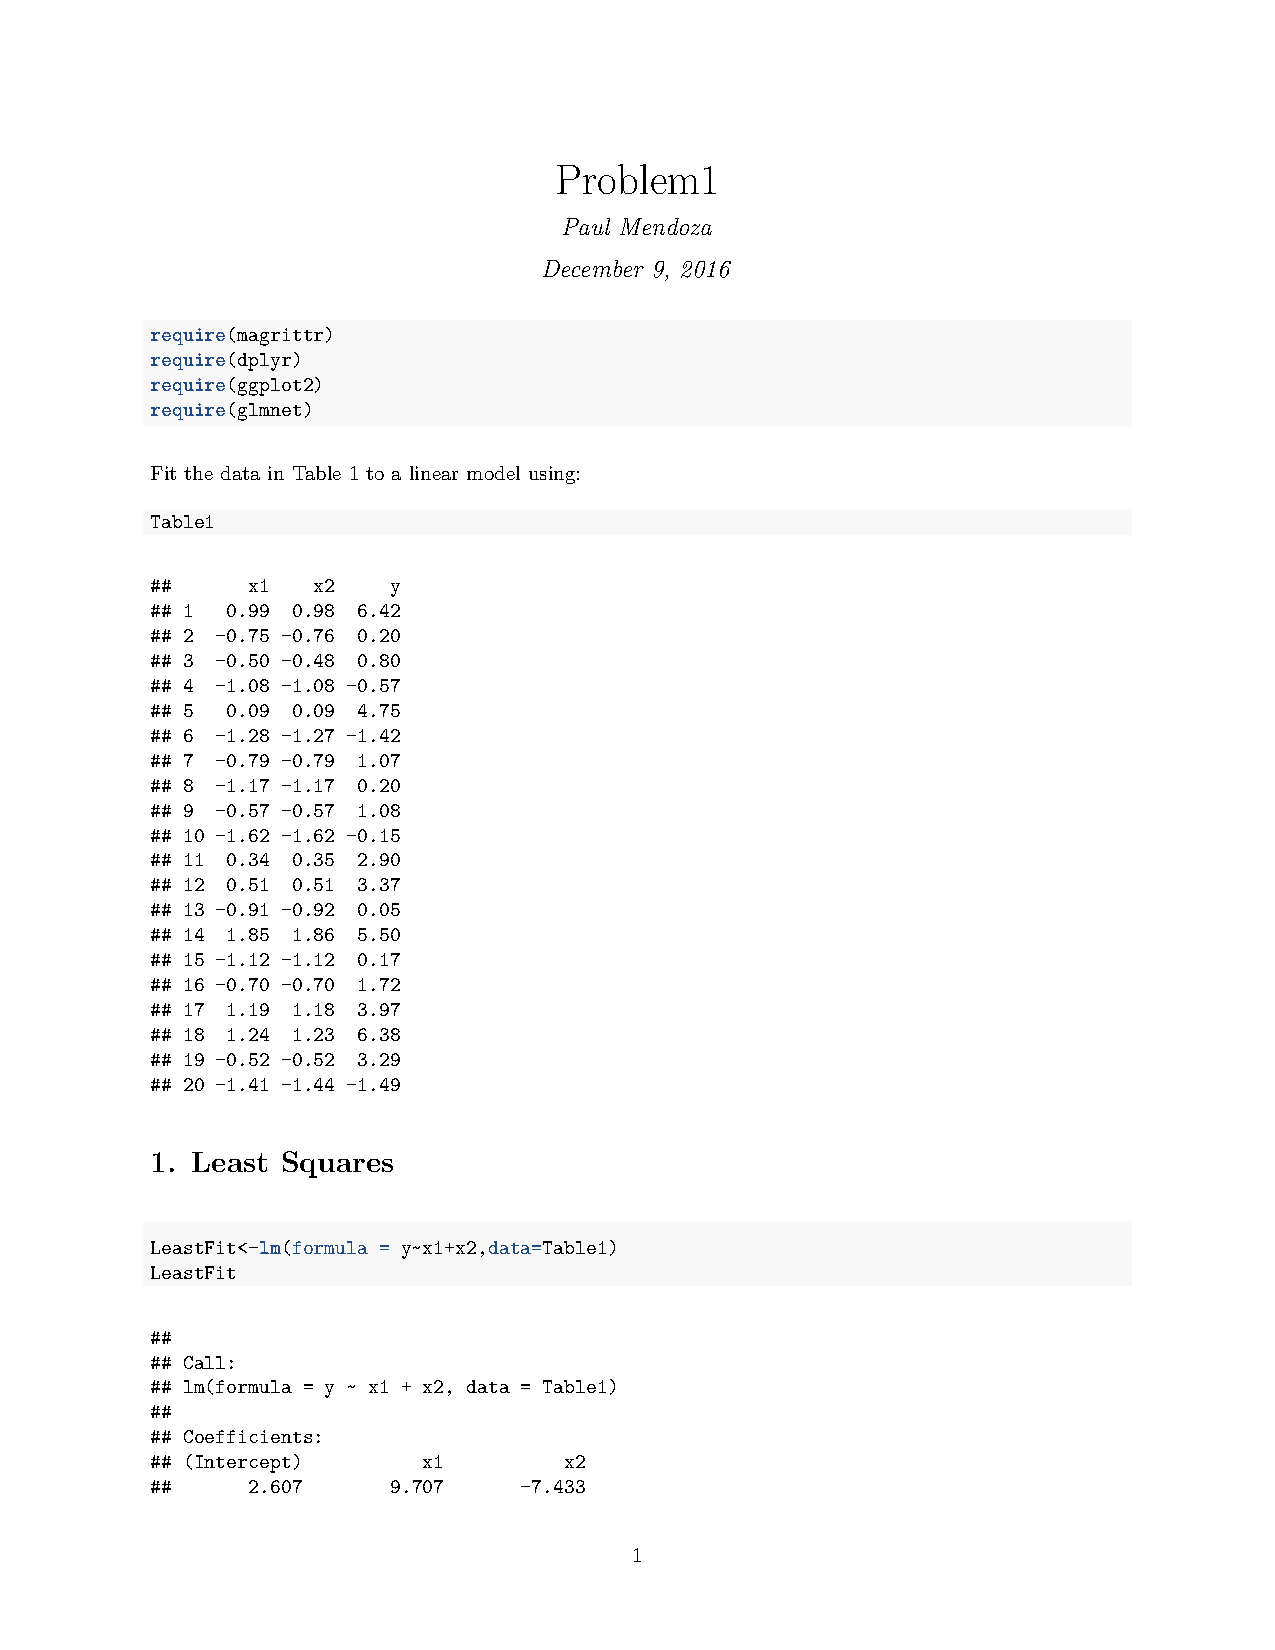
\includepdf[pages={1-10}]{Problem1_R/Problem1.pdf}
\end{homeworkProblem}

\clearpage



%--------------------------------------------------------------------------
%	PROBLEM 2
%--------------------------------------------------------------------------

\begin{homeworkProblem}
  Derive the adjoint operator for the equation
  \begin{equation*}
    -\bigtriangledown^2\phi(x,y,z)+\frac{1}{L^2}\phi(x,y,z)=\frac{Q}{D}
  \end{equation*}
  \begin{equation*}
    \phi(0,y,z)=\phi(x,0,z)=\phi(x,y,0)=\phi(X,y,z)=\phi(x,Y,z)
     =\phi(x,y,Z)=C
  \end{equation*}
  Compute the sensitivity to the QOI:
  \begin{equation*}
    QoI=\int_0^Xdx\int_0^Ydy\int_0^Zdz\ \frac{D}{L^2}\phi(x,y,z)
  \end{equation*}
  for X,Y,Z,L,D and Q.\\~\\

  \problemAnswer{
    \textbf{Derive the adjoint operator}\\~\\
    See Ch 6 for help more background. Define the operator $\mathcal{L}$ as
    \begin{equation*}
      \mathcal{L}=-D\bigtriangledown^2+\frac{D}{L^2}
    \end{equation*}
    and the adjoint $\mathcal{L^{\dag}}$ as
    \begin{equation*}
      \mathcal{L^{\dag}}=-D\bigtriangledown^2+\frac{D}{L^2}
    \end{equation*}
      \begin{equation*}
        \phi^\dag(0,y,z)=\phi^\dag(x,0,z)=
        \phi^\dag(x,y,0)=\phi^\dag(X,y,z)=\phi^\dag(x,Y,z)
     =\phi^\dag(x,y,Z)=C
      \end{equation*}
      Setting:
      \begin{equation*}
        \left|\frac{\delta\phi^\dag}{\delta x}\right|_{x=0}
        =
        \left|\frac{\delta\phi}{\delta x}\right|_{x=0}
      \end{equation*}
      and
      \begin{equation*}
        \left|\frac{\delta\phi^\dag}{\delta x}\right|_{x=X}
        =
        \left|\frac{\delta\phi}{\delta x}\right|_{x=X}
      \end{equation*}
      and similar for the other two dimentions.
    Also define the inner product as:
    \begin{equation*}
      (u,v)=\int_0^Xdx\int_0^Ydy\int_0^Zdz\ uv
    \end{equation*}
    
    \textit{Proof},
    in order to prove that this is an adjoint
    operator for the above equation, it needs to be shown that
    $(\mathcal{L}\phi,\phi^\dag)=(\phi,\mathcal{L}^\dag\phi^\dag)$.
    \\~\\
    Equivalent to (all terms have a $D$ in them and cancel):
    \begin{equation}
      \int_0^Xdx\int_0^Ydy\int_0^Zdz\left(-\phi^\dag
      \bigtriangledown^2\phi+\phi^\dag\frac{\phi}{L^2}\right)
      =
      \int_0^Xdx\int_0^Ydy\int_0^Zdz\left(-\phi\bigtriangledown^2\phi^\dag
      +\phi\frac{\phi^\dag}{L^2}\right)
    \end{equation}
    The terms
    \begin{equation*}
      \int_0^Xdx\int_0^Ydy\int_0^Zdz\left(\phi^\dag\frac{\phi}{L^2}\right)
      =
      \int_0^Xdx\int_0^Ydy\int_0^Zdz\left(\phi\frac{\phi^\dag}{L^2}\right)
    \end{equation*}
    are equal.
    For the other term with, $\bigtriangledown^2$, we can expand to
    (removing the negative sign for simplicity):
    \begin{equation*}
      \int_0^Xdx\int_0^Ydy\int_0^Zdz\left(
      \phi^\dag\left[
        \frac{\delta^2\phi}{\delta x^2}+
        \frac{\delta^2\phi}{\delta y^2}+
        \frac{\delta^2\phi}{\delta z^2}
      \right]
      \right)
    \end{equation*}
  }
  \problemAnswer{
    Focusing on the $x$ terms, noting that $y$ and $z$
    will have the same derivation. Integration by parts,
    with $u=\phi^\dag$,
    $du=\frac{\delta\phi^\dag}{\delta x}dx$, and
    $v=\frac{\delta\phi}{dx}$,
    $dv=\frac{\delta^2\phi}{\delta x^2}dx$ yields.

    \begin{align*}
      \int_0^Ydy\int_0^Zdz\left(
      \int_0^Xdx\ \phi^\dag\frac{\delta^2\phi}{\delta x^2}
      \right)=
      \int_0^Ydy\int_0^Zdz\left(
      \left|
      \phi^\dag\frac{\delta\phi}{\delta x}
      \right|_{x=0}^{x=X}
      -\int_0^Xdx\ \frac{\delta\phi}{\delta x}
      \frac{\delta\phi^\dag}{\delta x}dx
      \right)
    \end{align*}
  
  Performing another integration by parts,
  with $u=\frac{\delta\phi^\dag}{\delta x}$,
  $du=\frac{\delta^2\phi^dag}{\delta x} dx$ and,
  $v=\phi$, $dv=\frac{\delta \phi}{\delta x} dx$.
  \begin{align*}
      =\int_0^Ydy\int_0^Zdz\left(
      \left|
      \phi^\dag\frac{\delta\phi}{\delta x}
      \right|_{x=0}^{x=X}
      -\left|
      \phi\frac{\delta\phi^\dag}{\delta x}
      \right|_{x=0}^{x=X}
      +\int_0^Xdx\ \phi
      \frac{\delta^2\phi^\dag}{\delta x^2}dx
      \right)
  \end{align*}
  At the boundaries, both $\phi$ and $\phi^\dag$ are
  a constant, and the derivatives of both at the
  boundaries are equal, and therefore those terms cancel,
  leaving
  \begin{align*}
    \int_0^Ydy\int_0^Zdz\left(
      \int_0^Xdx\ \phi
      \frac{\delta^2\phi^\dag}{\delta x^2}dx
      \right)
  \end{align*}
  which is equal to the $x$ component of the $\bigtriangledown^2$
  term of the RHS of equation 1 above. 
  }


  \vspace{5mm}

  
  \problemAnswer{
    \textbf{Compute the sensitivity to the QoI:}\\~\\
    The QoI has been defined as,
    \begin{equation*}
      QoI=\int_0^Xdx\int_0^Ydy\int_0^Zdz\ \frac{D}{L^2}\phi(x,y,z)=
      (\phi,p),
    \end{equation*}
    with $p=\frac{D}{L^2}$. Recall the original system being,
    \begin{equation*}
      \mathcal{L}\phi=Q.
    \end{equation*}
    If we define an adjoint system as,
    \begin{equation*}
      \mathcal{L^{\dag}}\phi^\dag=p,
    \end{equation*}
    then the QoI can be represented as,
    \begin{equation*}
      QoI=(\phi,p)=(Q,\phi^\dag)
    \end{equation*}
    This is because,
    \begin{align*}
      (\mathcal{L}\phi,\phi^\dag)&=(\phi,\mathcal{L}^\dag\phi^\dag)\\
      (Q,\phi^\dag)&=(\phi,p)
    \end{align*}
    The first line was proved in the first part of the problem,
    and the second line substitutes $q$ for $\mathcal{L}\phi$
    on the LHS of the equation and $p$ for $\mathcal{L}^\dag\phi^\dag$
    on the RHS.

    If the solution for $\phi^\dag$ were known, then this problem
    would be a lot easier. Lets see if we can find it.
    \begin{align*}
      \mathcal{L^\dag}\phi^\dag&=p\\
      -D\bigtriangledown^2\phi^\dag+\frac{D}{L^2}\phi^\dag&=
      \frac{D}{L^2}\\
      \phi^\dag=1+L^2\bigtriangledown^2\phi^\dag
    \end{align*}
    Where the solution is $\phi^\dag=1+exp(\frac{x}{L})+exp(\frac{y}{L})
    +exp(\frac{z}{L})$
    }
  \problemAnswer{
    Now the QoI is, 
    \begin{align*}
      QoI&=(Q,\phi^\dag)\\
      &=\int_0^Xdx\int_0^Ydy\int_0^Zdz\ Q\phi^\dag\\
      &=\int_0^Xdx\int_0^Ydy\int_0^Zdz\ Q\left(
      1+e^{\frac{x}{L}}+e^{\frac{y}{L}}+e^{\frac{z}{L}}
      \right)\\
      &=QXYZ+QYZL(e^{X/L}-1)+QXZL(e^{Y/L}-1)+QXYL(e^{Z/L}-1)
    \end{align*}
  
    The sensitivity to the QoI will be determined with a simple
    derivative of the QoI with respect to particular variables.
    \begin{equation*}
      \frac{\delta QoI}{\delta X}
      =\boxed{QYZ+QYZe^{X/L}+QZL(e^{Y/L}-1)+QYL(e^{Z/L}-1)}
    \end{equation*}
    \begin{equation*}
      \frac{\delta QoI}{\delta Y}
      =\boxed{QXZ+QZL(e^{X/L}-1)+QXZe^{Y/L}+QXL(e^{Z/L}-1)}
    \end{equation*}
    \begin{equation*}
      \frac{\delta QoI}{\delta Z}
      =\boxed{QXY+QYL(e^{X/L}-1)+QXL(e^{Y/L}-1)+QXYe^{Z/L}}
    \end{equation*}
    \begin{equation*}
      \frac{\delta QoI}{\delta L}
      =\boxed{Q(YZe^{X/L}(1-e^{-X/L}-\frac{X}{L})
        +XZe^{Y/L}(1-e^{-Y/L}-\frac{Y}{L})
        +XYe^{Z/L}(1-e^{-Z/L}-\frac{Z}{L}))}
    \end{equation*}
    \begin{equation*}
      \frac{\delta QoI}{\delta D}=
      \boxed{0}
    \end{equation*}
    \begin{equation*}
      \frac{\delta QoI}{\delta Q}=
      \boxed{XYZ+YZL(e^{X/L}-1)+XZL(e^{Y/L}-1)+XYL(e^{Z/L}-1)}
    \end{equation*}
    }
\end{homeworkProblem}

\clearpage


%--------------------------------------------------------------------------
%	PROBLEM 3
%--------------------------------------------------------------------------

\begin{homeworkProblem}
  For the random variable X $\sim$ N(0,1) draw fifty samples
  and generate histograms using the following sampling
  techniques
  \begin{enumerate}[label=(\alph*)]
  \item{Simple random sampling}
  \item{Stratifid sampling}
  \item{A van der Corput sequence of base 2}
  \item{A van der Corput sequence of base 3}
  \end{enumerate}

  \problemAnswer{
    Simple random sampling samples U(0,1) and plugs this value
    into the inverse CDF. Stratified sampling separates U(0,1)
    into equal bins and samples ``Randomly'' in each bin.
    Van der Corput sequences divides an interval into a a
    number of equal subintervals.
    \\~\\
    For example, the ordinary van der Corput sequence in
    base 3 is given by 1/3, 2/3, 1/9, 4/9, 7/9, 2/9, 5/9, 8/9, 1/27.
  }

  \pythonscript{Problem3/Calculations}{Script for Problem}

  \begin{figure}[H]
    \begin{center}
      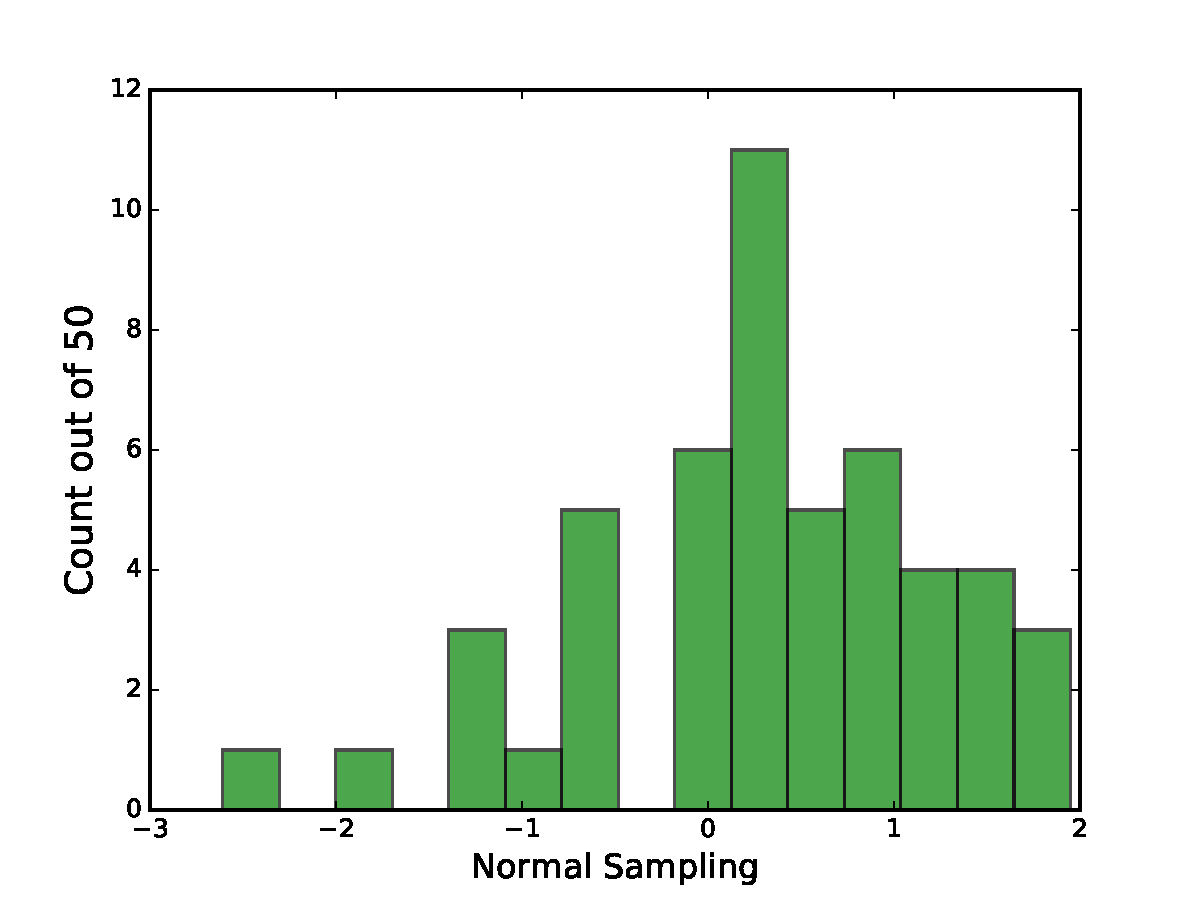
\includegraphics[width=0.77\columnwidth]{Problem3/NNorm.pdf}
    \end{center}
  \end{figure}

  \begin{figure}[H]
    \begin{center}
      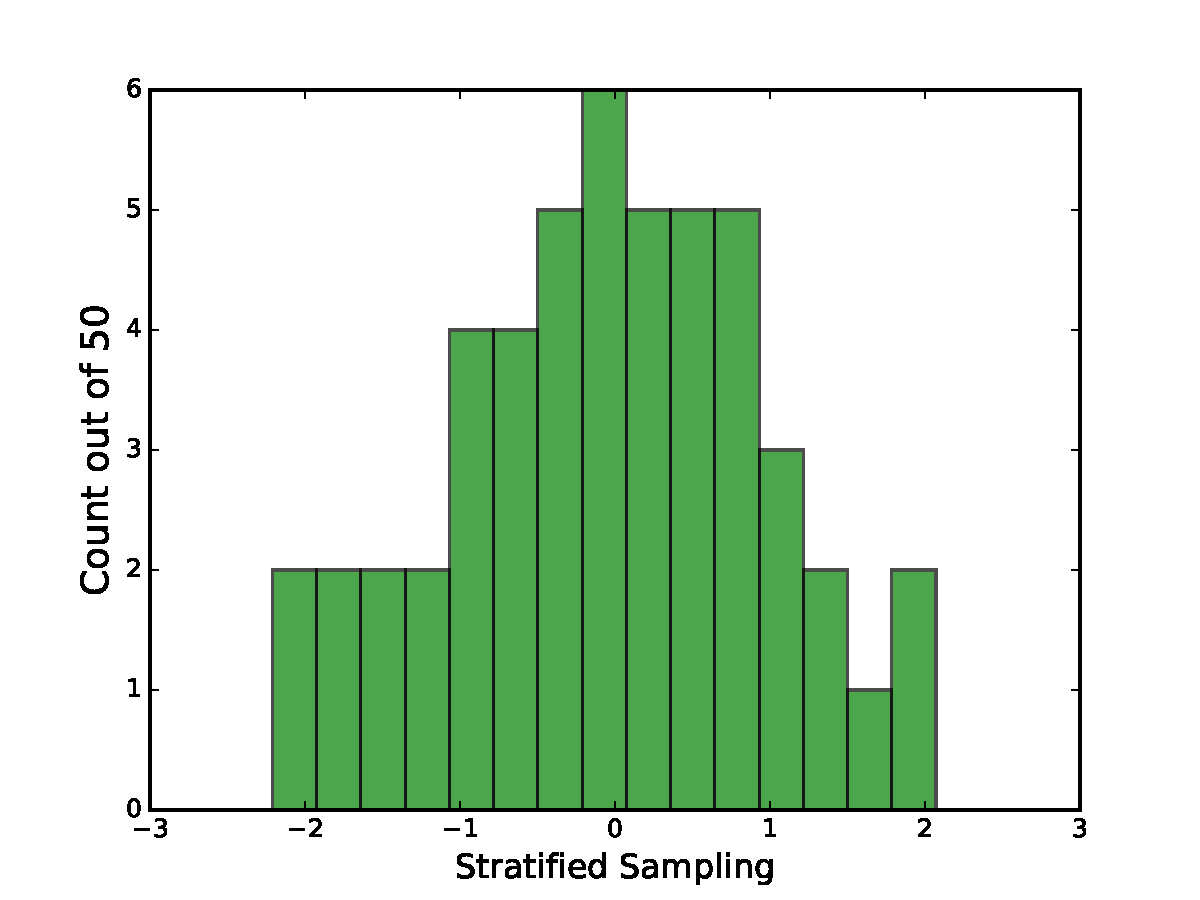
\includegraphics[width=0.77\columnwidth]{Problem3/SNorm.pdf}
    \end{center}
  \end{figure}

  \begin{figure}[H]
    \begin{center}
      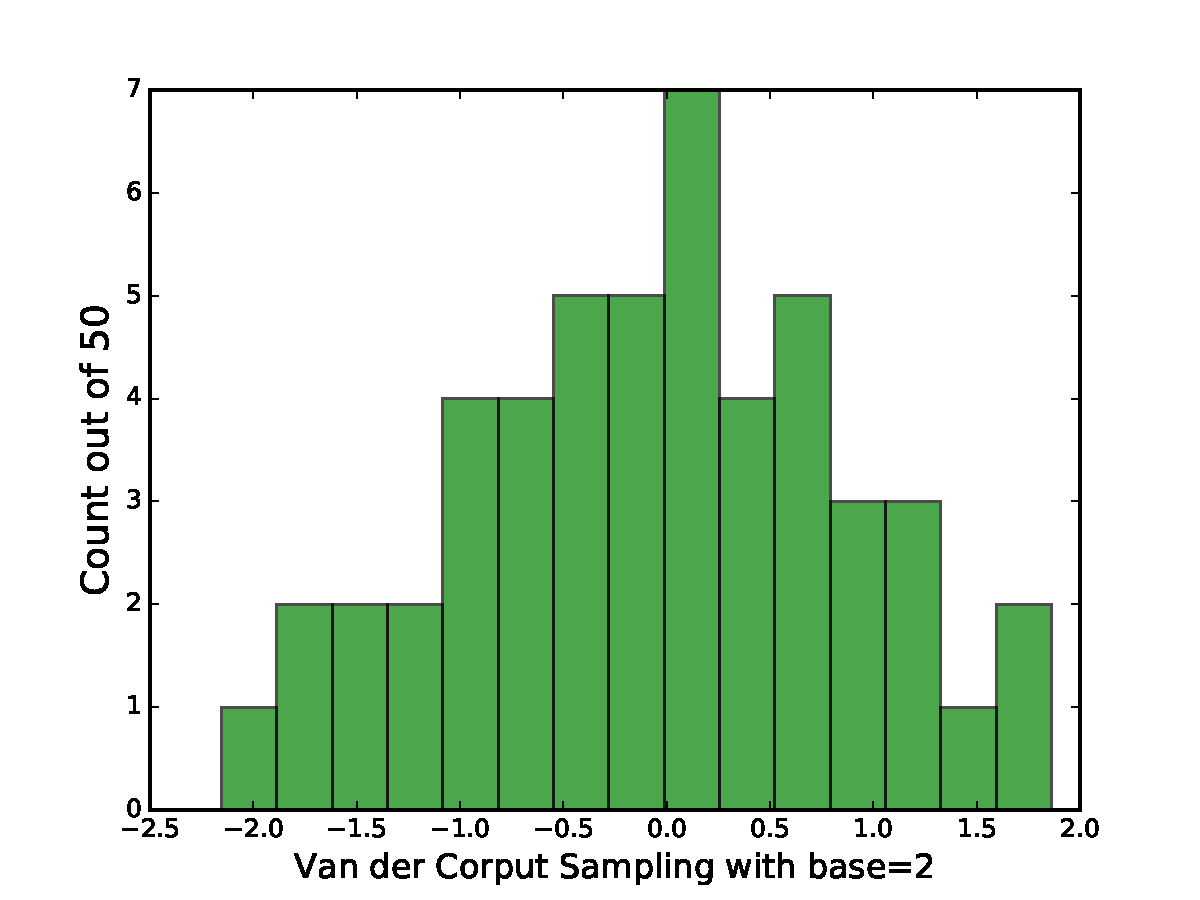
\includegraphics[width=0.77\columnwidth]{Problem3/V2Norm.pdf}
    \end{center}
  \end{figure}

  \begin{figure}[H]
    \begin{center}
      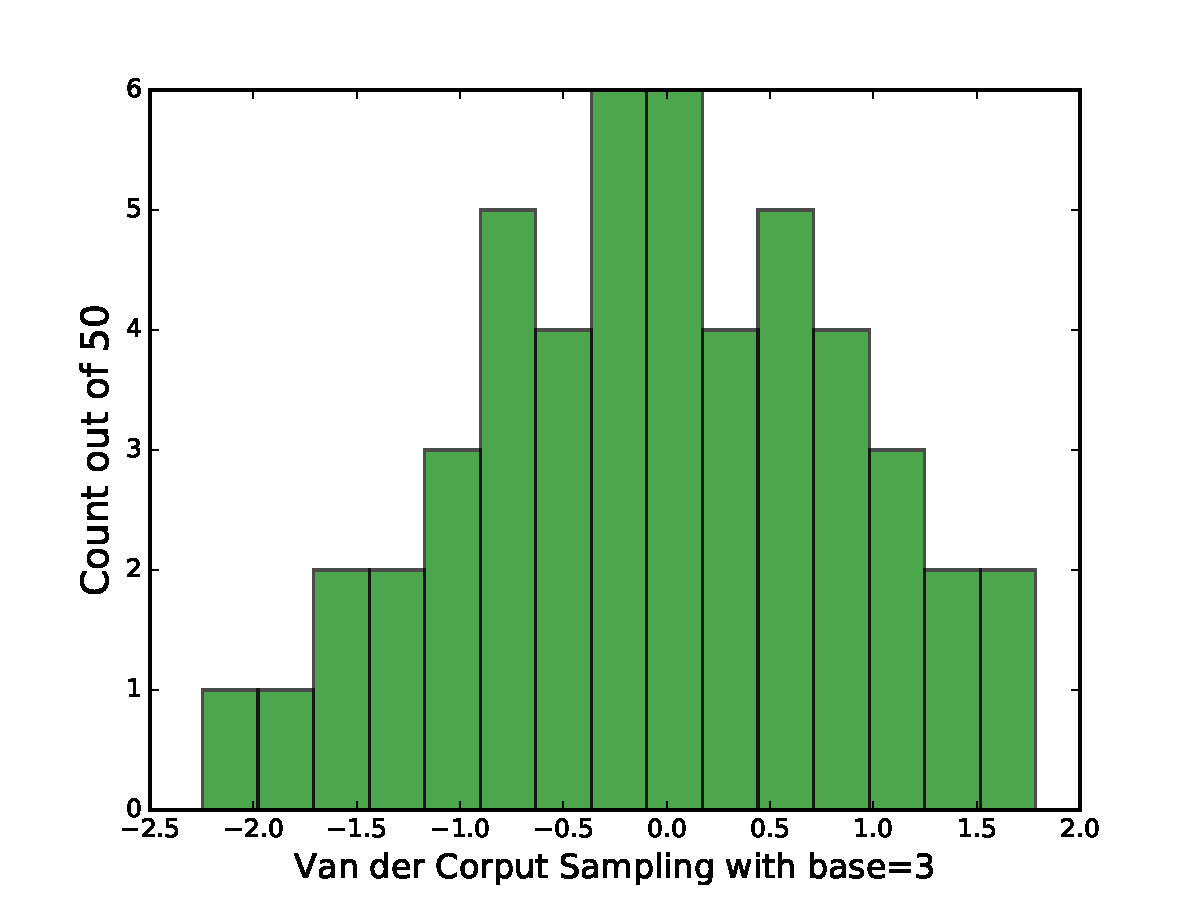
\includegraphics[width=0.77\columnwidth]{Problem3/V3Norm.pdf}
    \end{center}
  \end{figure}

\end{homeworkProblem}

\clearpage


%--------------------------------------------------------------------------
%	PROBLEM 4
%--------------------------------------------------------------------------

\begin{homeworkProblem}
  Consider the Rosenbrock function
  $f(x,y)=(1-x)^2+100(y-x^2)^2$. Assume that
  $x=2t-1$, where T $\sim\ B(3,2)$ and
  $y=2s-1$, where S $\sim\ B(1.1,2)$.
  Estimate the probability that $f(x,y)$ is
  less than 10 using:
  
  \begin{enumerate}[label=(\alph*)]
  \item{a first-order second-moment reliability method}
  \item{Latin hypercube sampling using 50 points}
  \item{A Halton sequence using 50 points}
  \end{enumerate}

  Compare this with the probability you calculate using
  10\tss{5} random samples. (\textit{Hint: Matlab has a
    built-in function for sampling beta R.V.'s ``betard''}).\\~\\

  \problemAnswer{
    \textbf{A first-order second-moment reliability method}\\~\\
    Will use a gaussian approximation as shown in section
    7.3 in the course notes (FORM).\\~\\

    In this method the performance function ($Z(x,y)$) is
    a function of the random variables $x$ and $y$, and
    is defined such that the failure surface is the location
    where $Z=0$ (top of page 119 Ch 7) such that $Z<0$
    represents failure and $Z>0$ represents success. For the
    case above, this would mean that our performance function
    is:
    
    \begin{align*}
      Z&=10-f(x,y)\\&=10-(1-x)^2-100(y-x^2)^2
    \end{align*}

    Next, the probability of failure is defined as:

    \begin{equation*}
      p_{fail}=1-\Phi\left(\frac{\mu_Z}{\sigma_Z}\right)
    \end{equation*}

    Where $\Phi$ is the CDF for a standard normal, $\mu_Z$ and
    $\sigma_Z$ are the mean and standard deviation of $Z$. As a
    reminder, if $Z$ were a standard normal, defined such
    that any part of $Z$ that is less than 0 is failure. Then
    because $\mu_Z=0$ there would be a 50\% chance of failure.
    If $Z$ were a non standard normal, then the distance from
    zero would be normalized (by dividing by $\sigma_Z$) to units
    of $\sigma$, and 
    as $\mu_Z$ increases, the chance of failure would continue
    to decrease, which make sense, as the mean of the
    performance function moves further and further away from
    the failure point ($Z=0$), the probability of failure decreases.
    \\~\\
    I am trying to spell this out for myself, because I was really
    confused about this.
    There are two things I would like to point out to future self.
    First, $Z$ may not be normal, which is why this method is only
    exact if $Z$ is normal, otherwise its an approximation. Second,
    if $\mu_Z$ were less than 0, then the equation for the
    probability of failure should (I think) change to

    \begin{equation*}
    p_{fail}=0.5+\Phi\left(\frac{|\mu_Z|}{\sigma_Z}\right)
    \end{equation*}

    Also third, I am not sure if $Z$ has to be a typical PDF
    or CDF, will let you know after I do some of the math McClarren
    gave.
  }
  \problemAnswer{
    The mean for $Z$ was defined as
    \begin{equation*}
      \mu_Z\approx g(\mu_{x,y})
    \end{equation*}
    where $g$ is the function we defined as $Z$ (first part of
    the taylor expansion of Z) evaluated at the mean values
    of $x$ and $y$. The standard
    deviation of $Z$ was defined as the the second part of the
    taylor expansion of $Z$ (without covariances because we
    are going to assume that all random variables are independent), namely

    \begin{equation*}
      \sigma_Z^2=
      \left(
      \left|\frac{\delta g}{\delta x}\right|_{\mu_x}\sigma_x
      \right)^2
      +
      \left(
      \left|\frac{\delta g}{\delta y}\right|_{\mu_y}\sigma_y
      \right)^2
    \end{equation*}
    
    For what I defined as $Z$ above,
    
    \begin{align*}
      \frac{\delta g}{\delta x}&=-2(x-1)-400x(x^2-y)\\
      \frac{\delta g}{\delta y}&=-200(y-x^2)
    \end{align*}
    Also for a beta R.V
    \begin{align*}
      \mu&=\frac{a}{a+b}\\
      \sigma^2&=\frac{ab}{(a+b)^2(a+b+1)}
    \end{align*}
  }
  \problemAnswer{
    \textbf{Calculations}\\~\\
    For the random variable $t$ used in $x=2t-1$
    \begin{center}
      mean
    \end{center}
    \begin{align*}
      \mu_t&=\frac{3}{3+2}=\bm{0.6}\\
      \mu_x&=2*\bm{0.6}-1=\boxed{0.2}
    \end{align*}
    \begin{center}
      standard deviation
    \end{center}
    \begin{align*}
      \sigma_t^2&=\frac{3\cdot2}{(3+2)^2(3+2+1)}=\bm{0.04}\\
      \sigma_x^2&=\left|
      \frac{\delta x}{\delta t}
      \right|_{\mu_T}^2\sigma_t^2\\
      &=2^2\cdot\bm{0.04}=\boxed{0.16}
    \end{align*}
  }
  \problemAnswer{
    For the random variable $s$ used in $y=2s-1$
    \begin{center}
      mean
    \end{center}
    \begin{align*}
      \mu_s&=\frac{1.1}{1.1+2}=\bm{0.354839}\\
      \mu_y&=2*\bm{0.354839}-1=\boxed{-0.290323}
    \end{align*}
    \begin{center}
      standard deviation
    \end{center}
    \begin{align*}
      \sigma_s^2&=\frac{1.1\cdot2}{(1.1+2)^2(1.1+2+1)}=\bm{0.055836}\\
      \sigma_y^2&=\left|
      \frac{\delta y}{\delta s}
      \right|_{\mu_s}^2\sigma_Ss^2\\
      &=2^2\cdot\bm{0.055836}=\boxed{0.223345}
    \end{align*}
  }
  \problemAnswer{
    For the partial derivative terms
    \begin{align*}
      \left|\frac{\delta g}{\delta x}\right|_{\mu_X}=
      -2(x-1)-400x(x^2-y)=-2(0.2-1)-400\cdot2(0.2^2-(-0.290323))=
      \boxed{-24.8258}
    \end{align*}

    \begin{align*}
      \left|\frac{\delta g}{\delta y}\right|_{\mu_y}=
      -200(y-x^2)=-200(-0.290323-0.2^2)=\boxed{66.0646}
    \end{align*}
  }
  \problemAnswer{
    For Z and the probability of failure

    \begin{align*}
      \mu_Z=10-(1-0.2)^2+100(-0.290323-0.2^2)^2=\boxed{20.2713}
    \end{align*}

    \begin{align*}
      \sigma_Z^2&=24.8^2\cdot0.16+66.0646^2\cdot0.223345=1073.41\\
      \sigma_Z&=\boxed{32.7629}
    \end{align*}

    \begin{align*}
      p_{fail}&=1-\Phi\left(\frac{20.27}{32.7629}\right)\\
      &=\boxed{\bm{0.268}}
    \end{align*}
  }
  \pythonscript{Problem4/Calculations}{Script for Hypercube and Halton}

  My PDF integrates to 1.01, which I'm okay with. The table below
  summarizes my results.

  \begin{table}[H]
    \begin{center}
      \caption{Different Sampling Techniques}
      \begin{tabular}{l l l}
        \toprule
        Method & $p_{fail}$ 50 points & $p_{fail}$ 100 points\\
        \hline
        Stratified & 0.30 & 0.28\\
        First Order & 0.268 & \\
        Latin Hyper & 0.36 & 0.26\\
        Halton & 0.24 & 0.25\\
        Normal (10\tss{5}) & 0.26017 &\\
        \bottomrule
      \end{tabular}
    \end{center}
  \end{table}
  
  It should be noted that I shuffled the stratified samples,
  because otherwise there would be some
  correlation between the numbers. The first order listing in the
  table is not from the code, but the calculation in the
  first part of the problem above (did not use 50 points). I
  realized I could have used a more complicated first-order
  second moment reliability method, but this is A reliability method.
  
  \begin{figure}[H]
    \begin{center}
      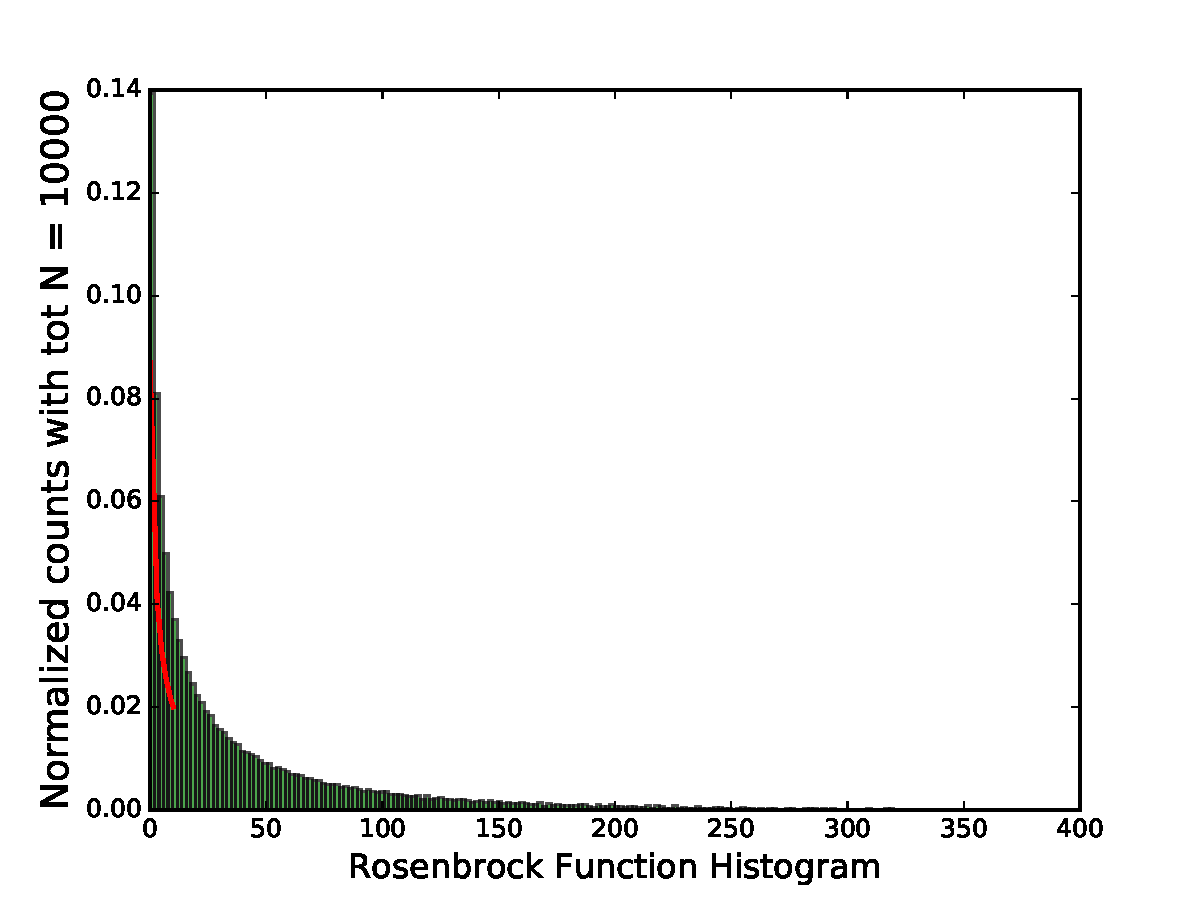
\includegraphics[width=0.77\columnwidth]{Problem4/Histf.pdf}
    \end{center}
  \end{figure}

    
  \begin{figure}[H]
    \begin{center}
      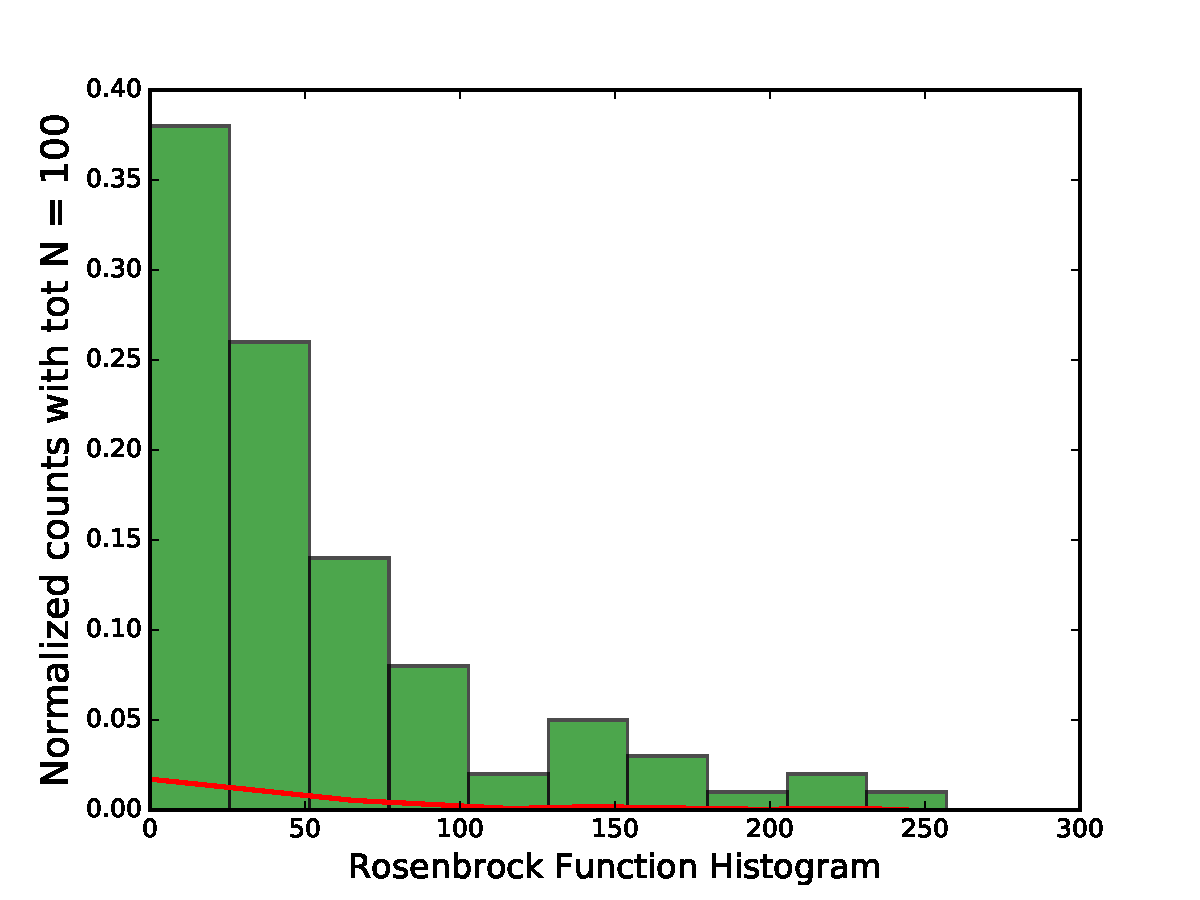
\includegraphics[width=0.77\columnwidth]{Problem4/HistLatin.pdf}
    \end{center}
  \end{figure}

  
\end{homeworkProblem}

\clearpage



%--------------------------------------------------------------------------
%	PROBLEM 5
%--------------------------------------------------------------------------

\begin{homeworkProblem}
  Consider the exponential integral function, $E_n(x)$,

  \begin{equation*}
    E_n(x)=\int_1^\infty \frac{e^{-xt}}{t^n}dt
  \end{equation*}

  This function is involved in the solution to many
  pure-absorbing transport problems. Use this function
  to solve the transport problem,

  \begin{equation*}
    \mu\frac{\delta\psi}{\delta x}+\sigma\psi=0,
  \end{equation*}

  \begin{equation*}
    \psi(0,\mu>0)=1, \psi(10,\mu<0)=0,
  \end{equation*}

  for the scaler flux $\phi(x)=\int_{-1}^1 \psi(x,\mu)d\mu$.
  Assume that $\sigma \sim\ GAM(10,0.1)$. Use a PCE
  expansion to estimate the distribution, mean, and
  variance of $\phi(x)$ at $x=1,1.5,3,5$. Also, plot
  the mean value of $\phi$ as a function of $x$.
  \\~\\
  \problemAnswer{

    Using the integrating factor approach we proceed as follows:

    \begin{align*}
      \frac{\delta\psi}{\delta x}+\frac{\sigma\psi}{\mu}&=0\\
      \frac{\delta}{\delta x}\left[
        e^{\frac{\sigma x}{\mu}}\psi
        \right]&=0\\
    \end{align*}
    Integrating from 0 to x for $\mu>0$, we obtain (yes I am copying
    some old notes)

    \begin{align*}
      \psi(x,\mu>0)e^{\frac{\sigma x}{\mu>0}}-\psi(0,\mu>0)
      e^{\frac{\sigma\cdot0}{\mu>0}}&=0\\
      \psi(x,\mu>0)e^{\frac{\sigma x}{\mu>0}}-1&=0\\
      \psi(x,\mu>0)e^{\frac{\sigma x}{\mu>0}}&=1\\
      \psi(x,\mu>0)&=e^{\frac{-\sigma x}{\mu>0}}
    \end{align*}

    Integrating from x to 10 for $\mu<0$, we obtain

    \begin{align*}
      \psi(10,\mu<0)e^{\frac{\sigma 10}{\mu<0}}-\psi(x,\mu<0)
      e^{\frac{\sigma\cdot x}{\mu<0}}&=0\\
      -\psi(x,\mu<0)
      e^{\frac{\sigma\cdot x}{\mu<0}}&=0\\
      \psi(x,\mu<0)&=0
    \end{align*}

    Here we can note that there is no flux traveling to the left,
    and will focus on the flux traveling to the right. Integrating
    over all $\mu>0$, and using a substitution of $z=1/\mu$ and
    $d\mu=-z^{-2}$:
  }
  \problemAnswer{
    \begin{align*}
      \phi^+(x)&=2\pi \int_0^1\psi(x,\mu>0)d\mu\\
      &=2\pi \int_0^1e^{-\frac{\sigma x}{\mu}}d\mu\\
      &=2\pi \int_\infty^1-\frac{e^{-\sigma xz}}{z^2}dz\\
      &=2\pi \int_1^\infty\frac{e^{-\sigma xz}}{z^2}dz\\
      &=2\pi E_2(\sigma x)
    \end{align*}
  }

  Now to use PCE expansion to estimate the distribution,
  mean, and variance of $\phi(x)$. First off, I want to say
  that I have no idea whats going on. Next, because we have a
  gamma distribution, I suppose we should use Laguerre Polynomials.
  Where:
  \begin{equation*}
    \phi(\sigma x)=2\pi \sum_{n=0}^{\infty}c_nL_n^{(\alpha)}
    (\beta x \sigma)
  \end{equation*}
  and
  \begin{equation*}
    c_n=2\pi \frac{n!}{\Gamma(n+\alpha+1)}\int_0^{\infty}
    E_2\left(\frac{x\cdot z}{\beta}\right)
    z^\alpha e^{-z}L_n^{(\alpha)}(z)dz
  \end{equation*}

  It should be noted that z is the standardized gamma distribution,
  with $z=\beta\sigma$, $\sigma$ being our original gamma distribution.\\
  
  In order to estimate the coefficients in the expansion we have to
  evaluate a wonderful integral. In order to estimate the integral, will
  use Gauss-Laguerre quadrature (like I have any idea what
  that is) to have as few evaluations of the integrand as possible.\\

  The quadrature rule has the form
  \begin{equation*}
    \int_0^\infty f(z)z^\alpha e^{-z}dz\approx
    \sum_{i=1}^{n}w_if(z_i)
  \end{equation*}

  Where $z_i$ are the n roots of $L_n^{(\alpha)}(z)$, and
  the weights are given by:

  \begin{equation*}
    w_i=\frac{\Gamma(n+\alpha)z_i}
    {n!(n+\alpha)(L_{n-1}^{\alpha}(z_i))^2}
  \end{equation*}

  Looking at the quadrature rule, I think $f(z)$, in our
  instance would have to be

  \begin{equation*}
    f(z)=E_2\left(\frac{x\cdot z}{\beta}\right)L_n^{(\alpha)}(z)
  \end{equation*}

  This is potentially confusing about the two n indice, so I'll
  put it all on one line, and hope its correct,
  if not then the only person I can
  blame is myself. The notes aren't very clear on what $f(z)$ is.

  \begin{align*}
    c_n&\approx\frac{n!}{\Gamma(n+\alpha+1)}
    \sum_{i=1}^{n'}w_if(z_i)\\
    c_n&\approx\frac{n!}{\Gamma(n+\alpha+1)}
    \sum_{i=1}^{n'}\frac{\Gamma(n'+\alpha)z_i}
        {n'!(n'+\alpha)(L_{n'-1}^{\alpha}(z_i))^2}
        E_2\left(\frac{x\cdot z_i}{\beta}\right)L_n^{(\alpha)}(z_i)\\
  \end{align*}
  Where $n'$ will increase until the summation is not changing,
  this is potentially confusing (for me). $n'$ will start at 1. At which
  point the Laguerre polynomial $L_1^\alpha(x)$ will have a single root.
  The 'summation' will be a single term. Then $n'$ will increase to 2,
  where there are two roots. The 'summation' will sum results from
  those two roots, \textbf{and not use the previous summation}
  (except to compare - not to add onto). The summation
  from $n'=1$ and $n'=2$ will be compared, if there is no difference
  (note there could be some zero terms)
  then the $n'$ stops increasing, and the most recent summation is what
  we use moving forward.\\

  Also $n$ is the constant we are solving for.
  This way, the $L_n^\alpha(z_i)$
  term on the right side will only be zero for when $n'=n$ (I hope
  this is correct).\\

  According to the notes, the variance is:

  \begin{equation*}
    \text{Var}(G)=\sum_{n=1}^{\infty}
    \frac{\Gamma(n+\alpha+1)}
    {\Gamma(\alpha+1)n!}c_n^2
  \end{equation*}

  And $c_0$ is:

  \begin{align*}
    c_0&=\int_0^\infty
    E_2\left(\frac{x\cdot z}{\beta}\right)
    \frac{z^\alpha e^{-z}}{\Gamma(\alpha+1)}dz
    =E[g(X)]\\
    &\approx\sum_{i=1}^{n'}\frac{\Gamma(n'+\alpha)z_i}
        {n'!(n'+\alpha)(L_{n'-1}^{\alpha}(z_i))^2}
        E_2\left(\frac{x\cdot z_i}{\beta}\right)\\
  \end{align*}

  To check if this is correct, we can change the $E_2$
  term for $cos(z/\beta)$ with Z $\sim$ G(1,2) and check to
  see if $c_n$ converge to what Dr. McClarren
  has in his notes...which I'm hoping are correct. 
  
  \pythonscript{Problem5/Calc}{Code for Calculation}

  
  \begin{table}[H]
    \begin{center}
      \caption{Compare to the Dr. MC}
      \begin{tabular}{l l l}
        \toprule
        $C_n$ & MC notes & Code\\
        \hline
        0 & 0.48 & 0.48 \\
        1 & 0.35 & 0.35 \\
        2 & 0.04 & 0.04 \\
        3 & -0.05 & -0.05 \\
        4 & -0.03 & -0.03 \\
        5 & -0.00 & -0.00 \\
        \bottomrule
      \end{tabular}
    \end{center}
  \end{table}

  I am glad that works, as soon as I try to extend this
  to our problem it broke down. The reason is, the example
  given in lecture, with cos(x) needs a modification on the
  $\alpha$ and $\beta$ terms so that my code gets the same
  answers ($\alpha+1$ and $1/\beta$). When working with the
  homework problem, the terms don't need the modification, and
  if we do modify, we get REALLY bad answers..Also it should
  be noted that I don't include the $2\pi$ in the code, but
  because these answers match up close with the next problem,
  I leave the $2\pi$ out.
  
  \begin{table}[H]
    \begin{center}
      \caption{Different Sampling Techniques}
      \begin{tabular}{l l l c}
        \toprule
        Location & Mean & Variance & Agree with MCNP\\
        \hline
        1   & 0.166714961646 & 0.00541820218281 & Yes\\
        1.5 & 0.090024688979 & 0.00303591212914 & Yes\\
        3   & 0.0192062954143 & 0.000475125069726 & Yes\\
        5   & 0.00362613412053 & 5.14761627202e-05 & Yes\\
        \bottomrule
      \end{tabular}
    \end{center}
  \end{table}

  
  \begin{figure}[H]
    \begin{center}
      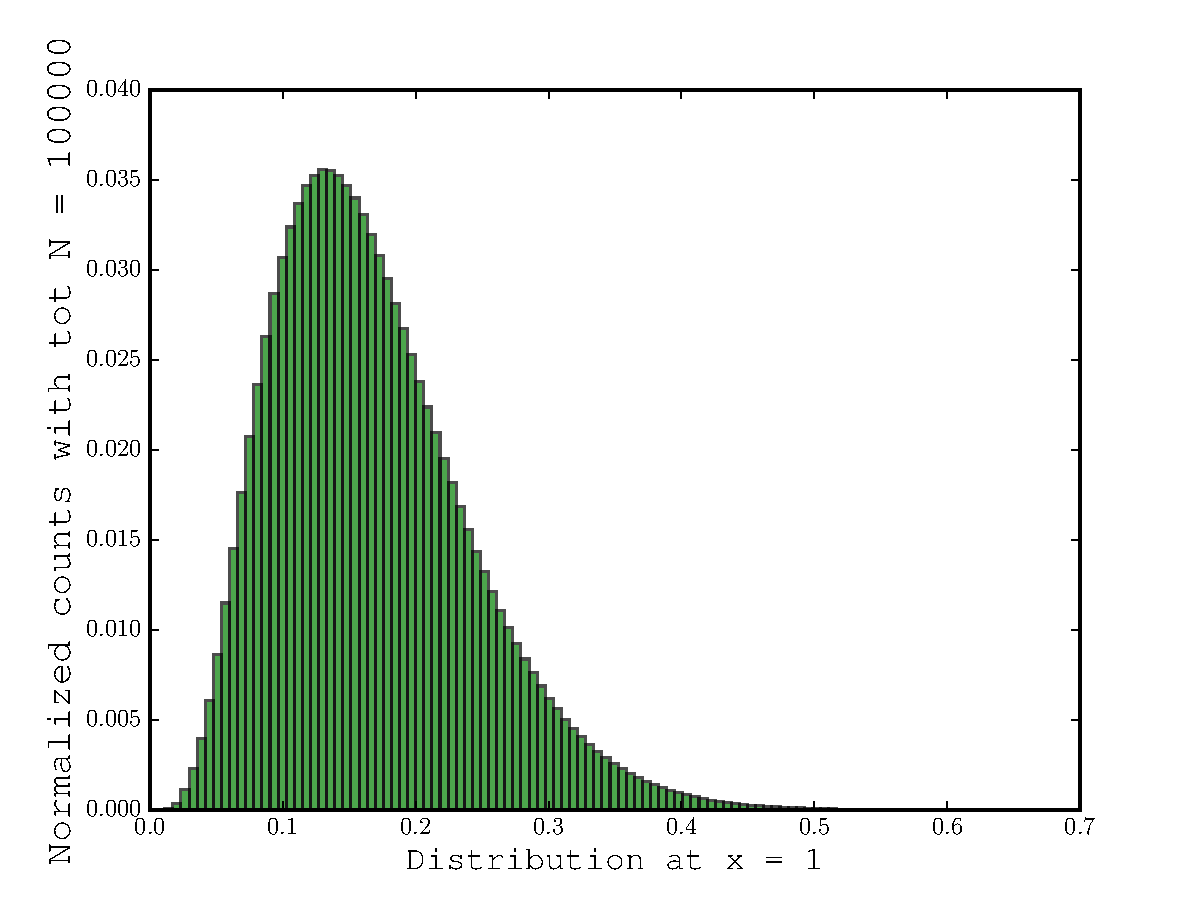
\includegraphics[width=0.77\columnwidth]{Problem5/meanx_1.pdf}
    \end{center}
  \end{figure}

  \begin{figure}[H]
    \begin{center}
      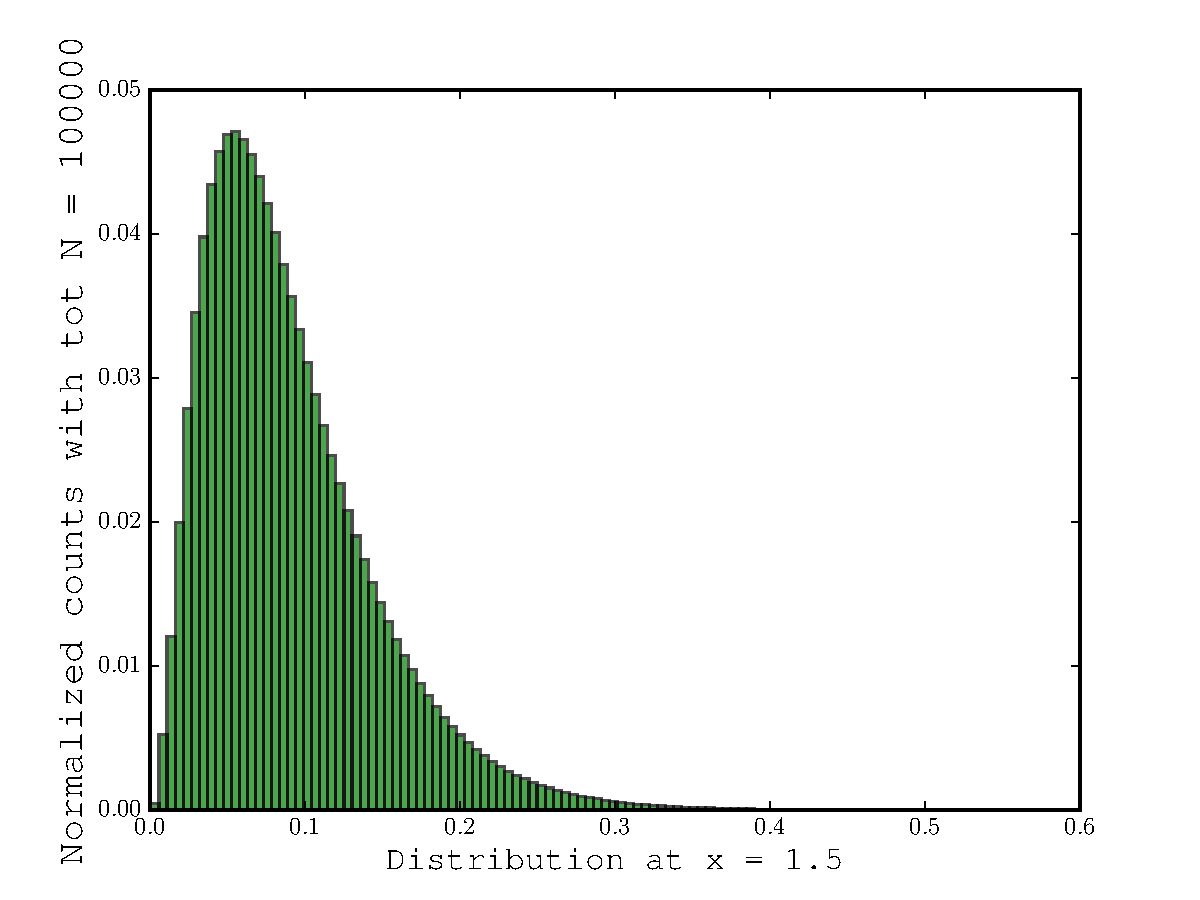
\includegraphics[width=0.77\columnwidth]{Problem5/meanx_15.pdf}
    \end{center}
  \end{figure}

  \begin{figure}[H]
    \begin{center}
      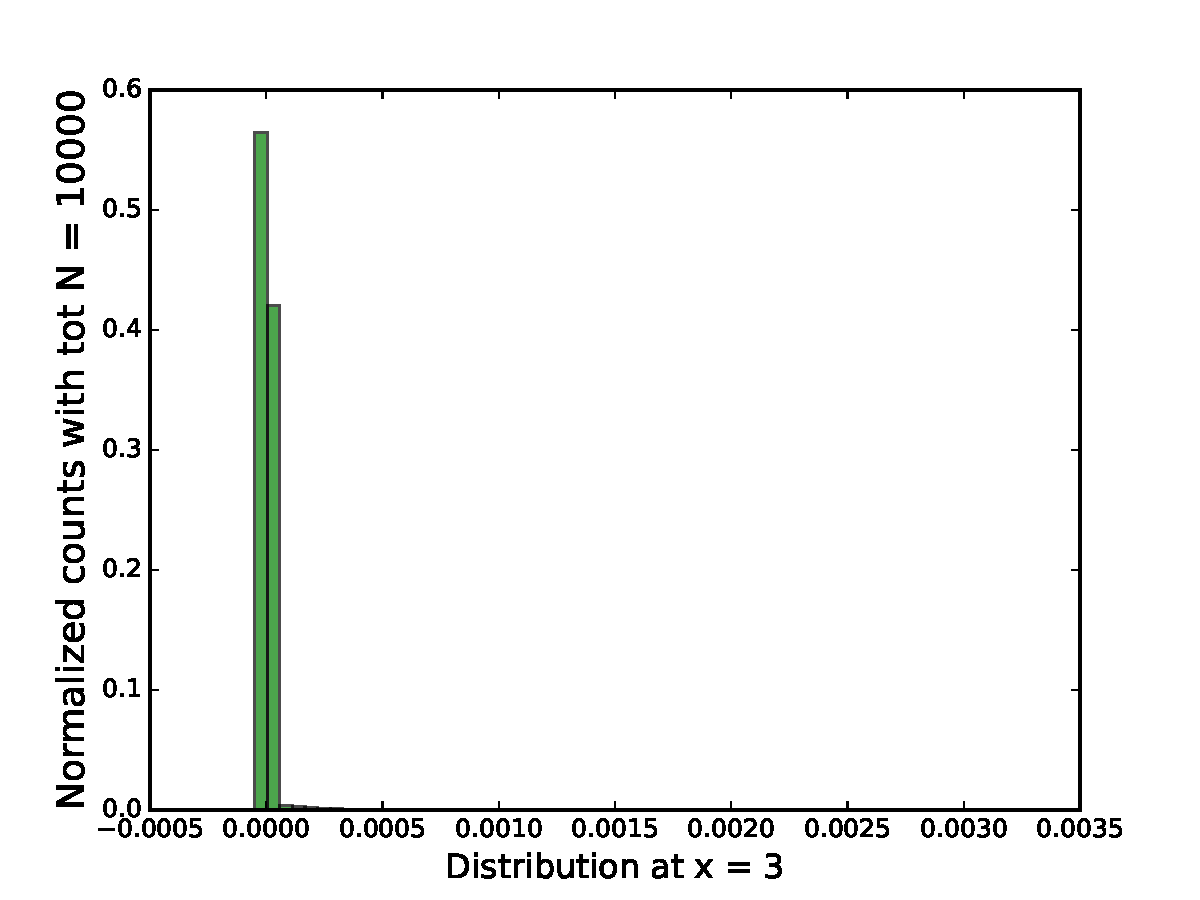
\includegraphics[width=0.77\columnwidth]{Problem5/meanx_3.pdf}
    \end{center}
  \end{figure}

  \begin{figure}[H]
    \begin{center}
      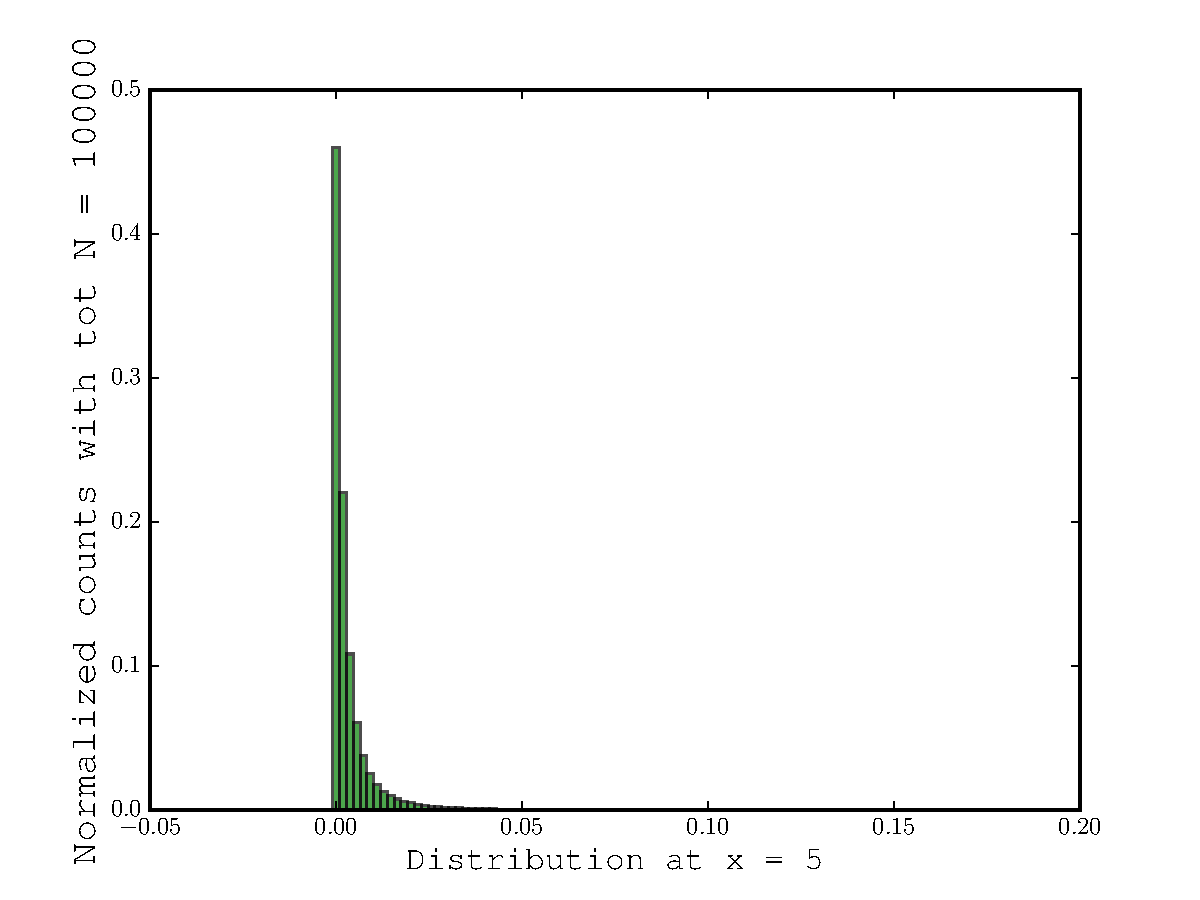
\includegraphics[width=0.77\columnwidth]{Problem5/meanx_5.pdf}
    \end{center}
  \end{figure}

  \pythonscript{Problem5/Calc}{Code for plot of mean as a function
  of x}
  
  Plot for the mean log scale and normal.
  \begin{figure}[H]
    \begin{center}
      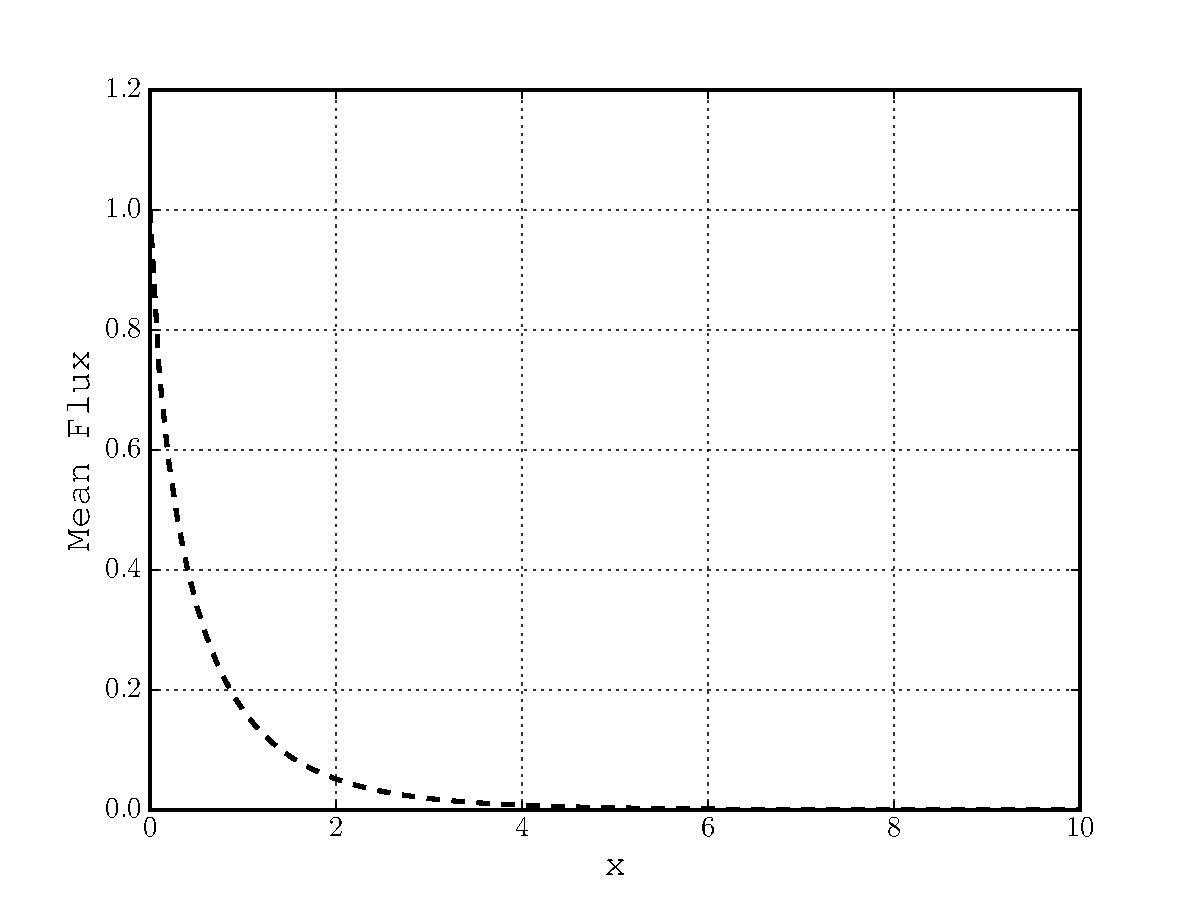
\includegraphics[width=0.77\columnwidth]{Problem5/mean.pdf}
    \end{center}
  \end{figure}
  \begin{figure}[H]
    \begin{center}
      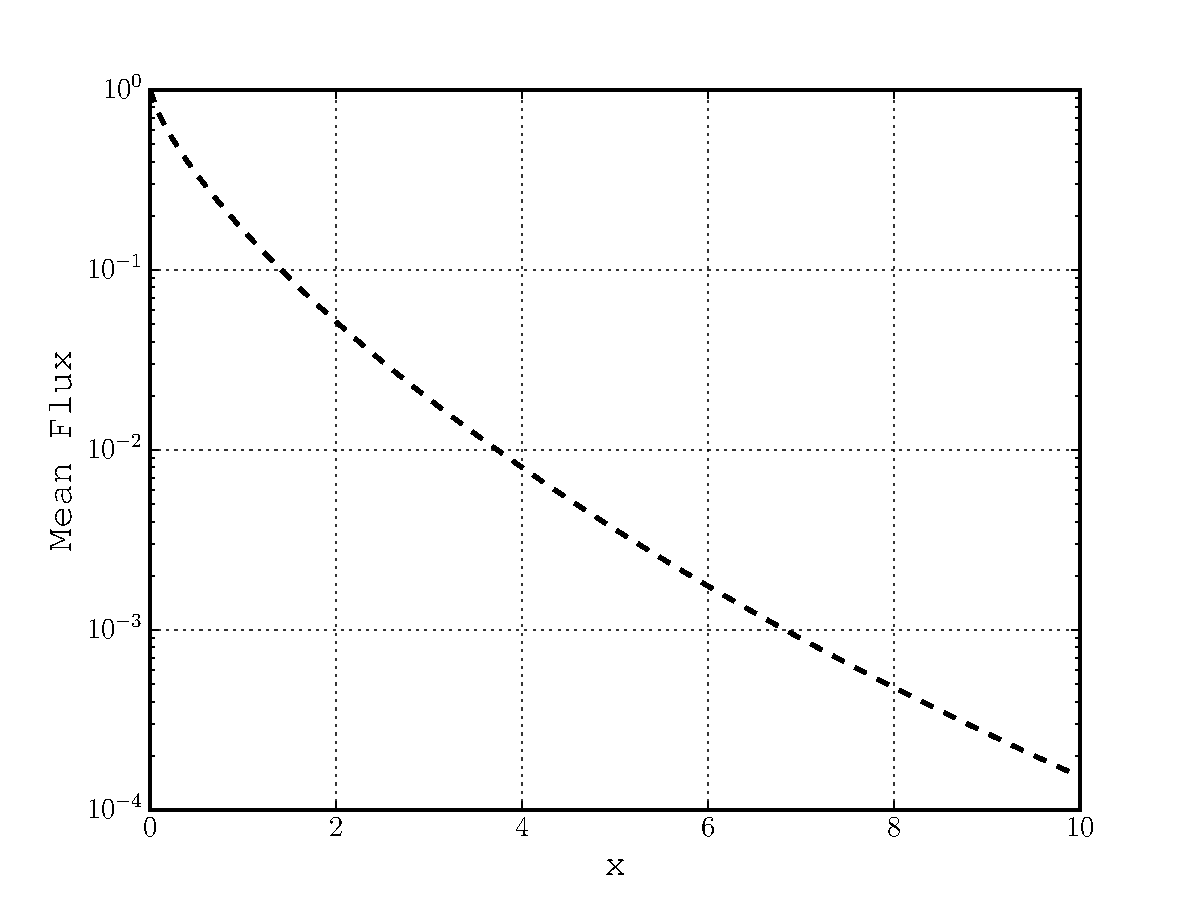
\includegraphics[width=0.77\columnwidth]{Problem5/meanlog.pdf}
    \end{center}
  \end{figure}

  
\end{homeworkProblem}



%--------------------------------------------------------------------------
%	PROBLEM 6
%--------------------------------------------------------------------------

\begin{homeworkProblem}
  You perform a measurement of a beam of radiation satisfying
  the boundary condition in problem 5 hitting a slab, and
  somehow are able to measure the scalar flux at $x=1,1.5,3,5$:

  \begin{table}[H]
    \begin{center}
      \caption{Measured and calculated flux}
      \begin{tabular}{l l l l}
        \toprule
        Location & Measured & Calculated & Variance\\
        \hline
        1   & 0.201131 & 0.166714961646 & 0.00541820218281\\
        1.5 & 110135 &  0.090024688979 & 0.00303591212914\\
        3   & 0.0228748 & 0.0192062954143 & 0.000475125069726\\
        5   & 0.0032849 & 0.00362613412053 & 5.14761627202e-05\\
        \bottomrule
      \end{tabular}
    \end{center}
  \end{table}

  
  Using the prior distribution for $\sigma$ from problem 5,
  and the experimental data just given, derive a posterior
  distribution for $\sigma$ (i.e calibrate $\sigma$). You
  may assume that the measurement has an error distributed by
  N(0,$\sigma$=0.001).\\~\\

  \problemAnswer{
    It should be noted that I might not have time to get to
    this problem, although it looks like it might be simple.
    
  }
  
\end{homeworkProblem}

\clearpage



%--------------------------------------------------------------------------
%	PROBLEM 1 Long
%--------------------------------------------------------------------------

\begin{homeworkProblem}[Long Problem 1]
  Using a discretization of your choice, solve the equation
  \begin{equation*}
    \frac{\delta u}{\delta t}+v\frac{\delta u}{\delta x}=
    D\frac{\delta^2u}{\delta x^2}-\omega u
  \end{equation*}
  for $u(x,t)$ on the spatial domain $x\in[0,10]$ with periodic
  boundary conditions $u(0^-)=u(10^+)$ , and initial conditions
  \begin{equation*}
    u(x,0)=
    \begin{cases}
      1, & x\in[0,2.5]\\
      0, & \text{otherwise}
    \end{cases}
  \end{equation*}
  Use the solution to compute the total reactions. 
  \begin{equation*}
    \int_5^6dx\int_0^5 dt\ \omega u(x,t).
  \end{equation*}
  Compute scaled sensitivity coefficients and sensitivity indices
  for normal random variables:
  \begin{enumerate}[label=(\alph*)]
  \item{$\mu_v=0.5,\ \sigma_c=0.1$}
  \item{$\mu_D=0.125,\ \sigma_D=0.03$}
  \item{$\mu_\omega=0.1,\ \sigma_\omega=0.05$}
  \end{enumerate}
  How do these results change with changes in $\Delta x$ and $\Delta t$?\\~\\
  There are scanned notes attached to this document as supplementary
  work. The code for calculating the reaction rate is shown below and
  is used for problems 3, and 4, but is only shown here.
  Specific code for other calculations will be shown.
  
  \pythonscript{Problem1_long/Calculations}{Code for RXNs}

  \problemAnswer{
    \vspace{3mm}
    Scanned Notes at the end of document.\\~\\

    The scaled sensitivity coefficient, and sensitivity
    index are defined as
    \begin{equation*}
      \text{Scaled Sensitivity Coeff}|_i=
      \left|\mu_i\frac{\delta\text{QoI}}
               {\delta\theta_i}\right|_{\bar{\theta}}
    \end{equation*}
    \begin{equation*}
      \text{Sensitivity Index}|_i=
      \left|\sigma_i\frac{\delta\text{QoI}}
               {\delta\theta_i}\right|_{\bar{\theta}}
    \end{equation*}
    Where the QoI is evaluated at mean values for parameters and
    a single parameter is varied off the mean.

    The code for calculating these values is shown below
    }
    \pythonscript{Problem1_long/Calc2}{Code for Sensitivities}

  \begin{table}[H]
    \begin{center}
      \caption{Sensitivity Parameters dx = 0.1 dt = 0.5}
      \begin{tabular}{l l l}
        \toprule
        Parameter & Scaled Sensitivity Coeff & Sensitivity Index\\
        \hline
        $v$       &  0.0668156428348 & 0.013363128567 \\
        $D$       &  0.00872948872873 & 0.0020950772949 \\
        $\omega$  &  0.0114146347046 & 0.00570731735231 \\
        \bottomrule
      \end{tabular}
    \end{center}
  \end{table}
    
  \begin{figure}[H]
    \begin{center}
      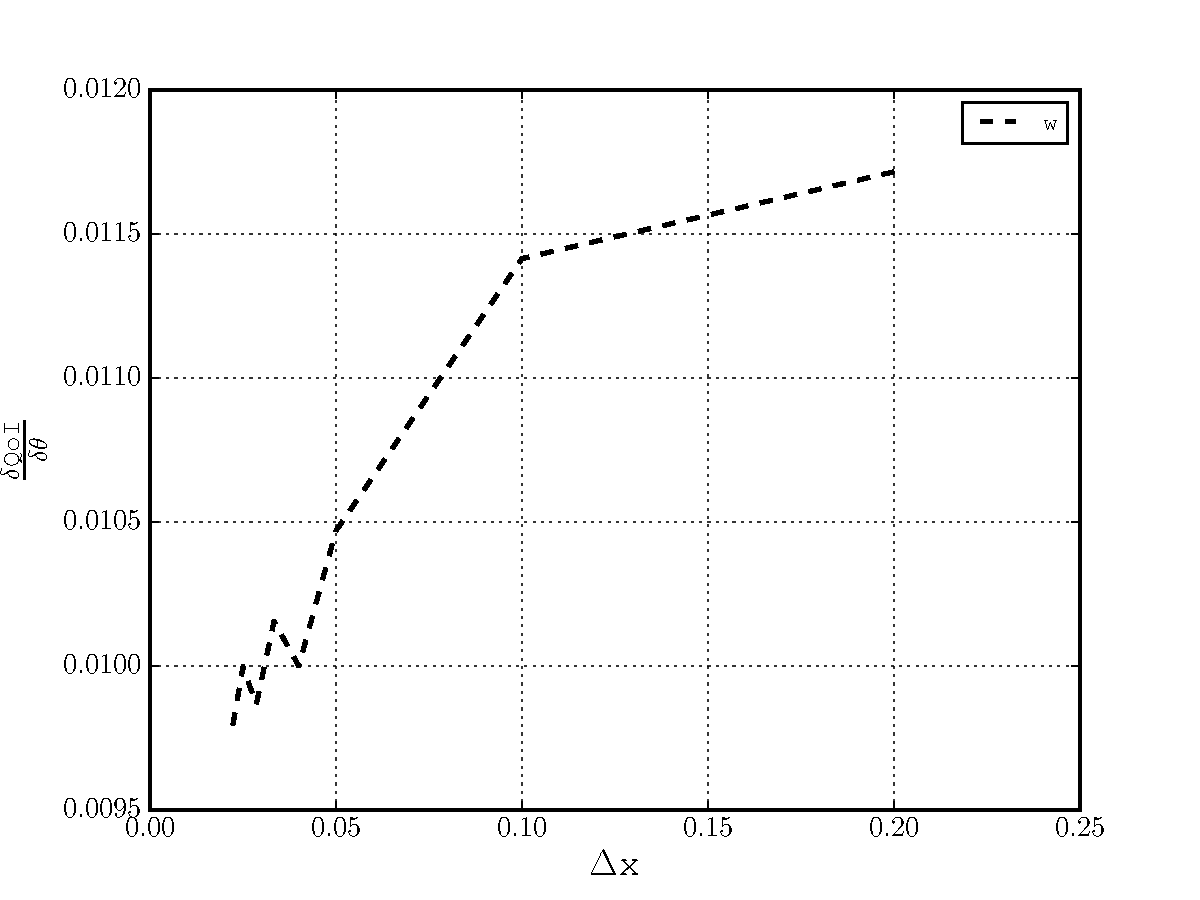
\includegraphics[width=0.77\columnwidth]{Problem1_long/scaled.pdf}
    \end{center}
  \end{figure}
  \begin{figure}[H]
    \begin{center}
      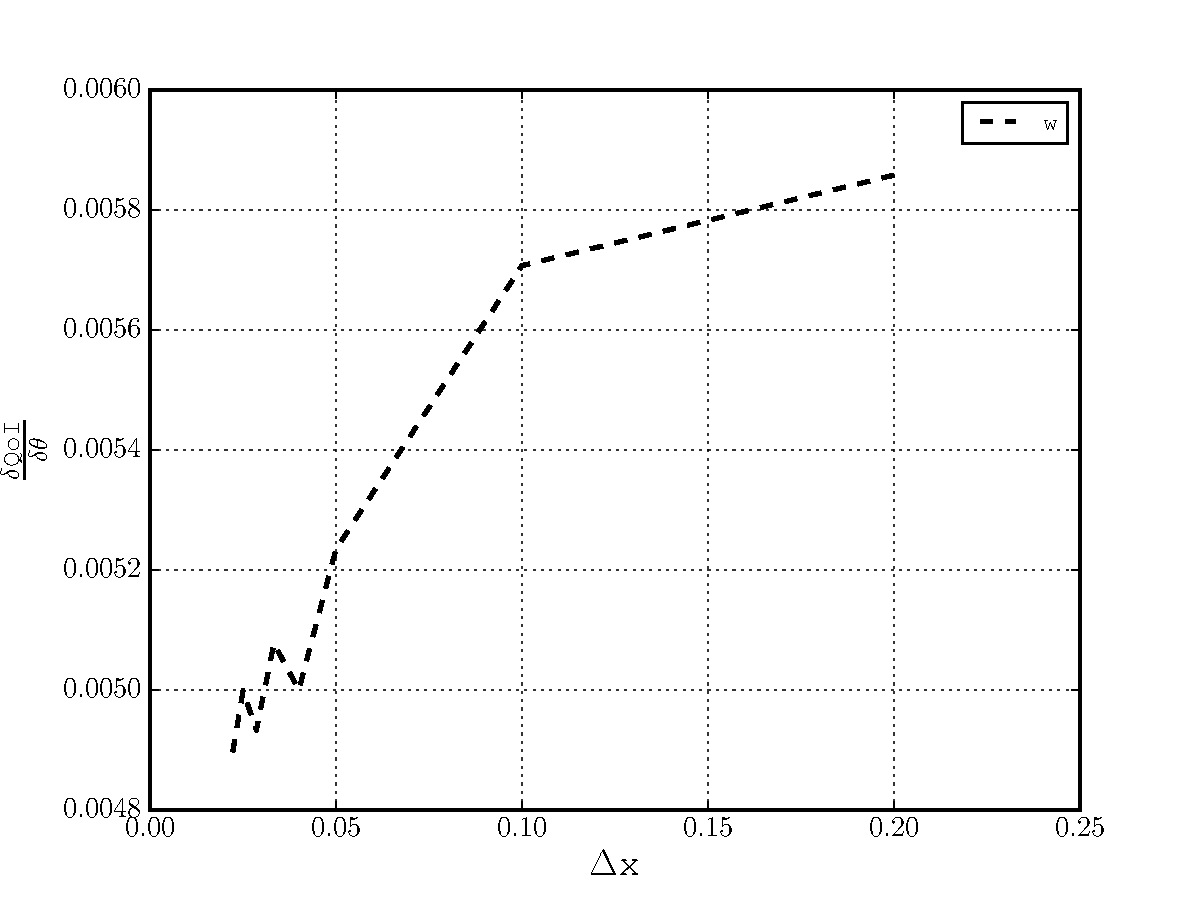
\includegraphics[width=0.77\columnwidth]{Problem1_long/index.pdf}
    \end{center}
  \end{figure}
  
\end{homeworkProblem}

\clearpage



%--------------------------------------------------------------------------
%	PROBLEM 3 Long
%--------------------------------------------------------------------------

\begin{homeworkProblem}[Long Problem 3]
  Using a discretization of your choice, solve the equation
  \begin{equation*}
    \frac{\delta u}{\delta t}+v\frac{\delta u}{\delta x}=
    D\frac{\delta^2u}{\delta x^2}-\omega u
  \end{equation*}
  for $u(x,t)$ on the spatial domain $x\in[0,10]$ with periodic
  boundary conditions $u(0^-)=u(10^+)$ , and initial conditions
  \begin{equation*}
    u(x,0)=
    \begin{cases}
      1, & x\in[0,2.5]\\
      0, & \text{otherwise}
    \end{cases}
  \end{equation*}
  Use the solution to compute the total reactions
  \begin{equation*}
    \int_5^6dx\int_0^5 dt\ \omega u(x,t).
  \end{equation*}
  Sample values of parameters using a uniform distribution
  centered at the mean with upper and lower bounds $\pm10\%$
  for the following variables:
  \begin{enumerate}[label=(\alph*)]
  \item{$\mu_v=0.5$}
  \item{$\mu_D=0.125$}
  \item{$\mu_\omega=0.1$}
  \end{enumerate}
  and sample values of the following parameters in their given ranges:
  \begin{enumerate}[label=(\alph*)]
  \item{$\Delta x \sim [0.001,0.5]$}
  \item{$\Delta t \sim [0.001,0.5]$}
  \end{enumerate}
\end{homeworkProblem}

\clearpage


%--------------------------------------------------------------------------
%	PROBLEM 4 Long
%--------------------------------------------------------------------------

\begin{homeworkProblem}[Long Problem 4]
  Using a discretization of your choice, solve the equation
  \begin{equation*}
    \frac{\delta u}{\delta t}+v\frac{\delta u}{\delta x}=
    D\frac{\delta^2u}{\delta x^2}-\omega u
  \end{equation*}
  for $u(x,t)$ on the spatial domain $x\in[0,10]$ with periodic
  boundary conditions $u(0^-)=u(10^+)$ , and initial conditions
  \begin{equation*}
    u(x,0)=
    \begin{cases}
      1, & x\in[0,2.5]\\
      0, & \text{otherwise}
    \end{cases}
  \end{equation*}
  Use the solution to compute the total reactions
  \begin{equation*}
    \int_5^6dx\int_0^5 dt\ \omega u(x,t).
  \end{equation*}
  Compute the probability that this quantity of interest is greater
  than 0.035 using LHS sampling of 50 points, 50 points of a
  Halton sequence, and a first-order second moment method using the
  following distributions
  \begin{enumerate}[label=(\alph*)]
  \item{$\mu_v=0.5,\ \sigma_c=0.1$}
  \item{$\mu_D=0.125,\ \sigma_D=0.03$}
  \item{$\mu_\omega=0.1,\ \sigma_\omega=0.05$}
  \end{enumerate}
  How do these results change with changes in $\Delta x$ and $\Delta t$?

\end{homeworkProblem}

\clearpage






%\pythonscript{Problem1/Calculations}{Script for Problem}
%% \begin{figure}[H]
%%   \begin{center}
%%     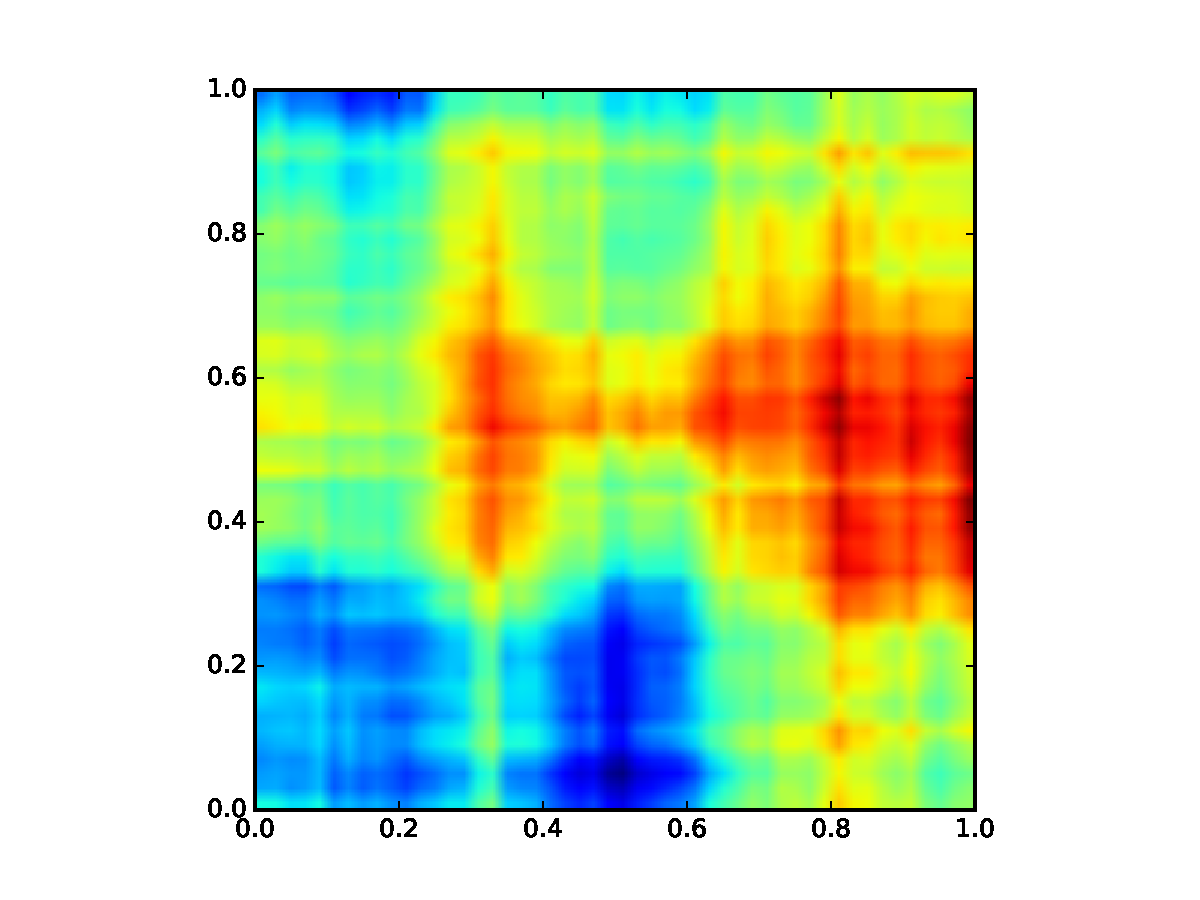
\includegraphics[width=0.77\columnwidth]{Problem1/P1realization1.pdf}
%%   \end{center}
%% \end{figure}
%\problemAnswer{TADA}

%--------------------------------------------------------------------------
%% This is an example citation \cite{Tatro2013}.
%% \bibliography{references} 
%% \bibliographystyle{plain} 

\end{document}
